\chapter{Machinelles Lernen}

Der Themenbereich des \keyword{Machinellen Lernens} beschäftigt sich mit Algorithmen und mathematischen Modellen, welche von selber lernen, Probleme zu loesen.
Hierbei wird nicht explizit einprogrammiert, wie das Modell das Problem zu loesen
hat, statdessen wird das Modell trainiert, optimiert sich von selbst und findet selber
einen Weg, das Problem zu loesen.
Die Grundidee dabei ist, dass man Daten erfasst, generiert oder misst, welche
analysiert werden sollen. Innerhalb diesen Daten existieren gewisse
Gesetzmaessigkeiten und Mustern. Diese Muster sollen vom Modell
erkannt werden und verallgemeinert werden. Nach dem erfolgreichen Lernen,
kann das Modell \keyword{Vorhersagen} zu neuen Daten machen.
\para{}
Man unterscheiden zwischen zwei Arten von Maschinellen Lernen:
\begin{itemize}
\item{
    \keyword{Ueberwachtes Lernen} (engl.:\ supervised learning) ist ein
    Lernverfahren, bei welchem die Daten aus zwei Teilen bestehen, aus Inputs und
    Outputs. Man bezeichnet dabei die Outputs als Labels. Die Aufgabe des Modells
    ist es eine \keyword{Korrelation} zwischen den Inputs und den Labels zu
    erlernen und so ihre Beziehung zueinander zu verstehen.
    Anhand der Informationen, welche in den Inputs enthalten
    sind, sind dann die Labels vorherzusagen. Man gleicht dann die
    vorhergesagten Labels des Modells mit den wahren Labels ab (man ueberwacht sie) und bewertet so ihre Faehigkeiten.
    \para{}
    Voraussetztung dafuer ist, dass die Daten eben ``gelabelt'' sein muessen.
    Man muss schon im vorhinein Daten haben, bei welchen man die gewuenschten
    Labels hat. Natuerlich muss auch die erwaehnte Korrelation bestehen. Falls
    kein Zusammenhang zwischen den Inputs und den Outputs besteht, kann das
    Modell auch keine Vorhersagen machen und so auch nichts erlernen.
  }
\item{
    \keyword{Unueberwachtes Lernen} (engl.:\ unsupervised learning) ist ein anderes
    Lernverfahren, bei welchem eben diese Labels nicht vorhanden sind. Dem
    Modell stehen nur die Inputdaten zur Verfuegung. Diese werden erneut analyisert
    und das Modell soll Muster herausextrahieren, welche sich von sonstigem
    zuefaelligen Rauschen (durch z.B. Messungenauigkeiten erzeugt)
    unterscheiden.
  }
\end{itemize}

Der Grossteil der Modelle des Maschinellen Lernens benutzten ueberwachtes
Lernen, da es auch deutlich mehr Anwendungsmoeglichkeiten besitzt. Es gibt nur wenige Arten von
unueberwachtem Lernen, darunter sind: Hauptkomponentenanalyse und Generative
Adversial Networks. Aus diesem Grund, werden wir im folgenden uns grundsaetzlich
mit ueberwachtem Lernen beschaeftigen. \\
Im Verlauf dieser Arbeit, werden auch noch Autoencoder betrachten, welche eine
Art Mischform darstellen. Man spricht von semiueberwachtem Lernen.
\para{}

Um die neuen Konzepte in den folgenden Abschnitten besser zu verstehen, werden
wir ein bestimmtes Beispielmodell betrachten:\\
Das Ziel ist den Preis eines Occasion Autos vorherzusagen, anhand der Anzahl
gefahrener Kilometer und anhand des Alters des Autos.

\para{}
\cite{wiki:supervised_learning}
\cite{wiki:unsupervised_learning}

\section{Allgemeine Begriffe}

\subsection{Daten}

Um ein Modell zu trainieren braucht man Daten. Diese Daten bestehen immer aus
\keyword{Inputs} und aus \keyword{Outputs}. Man unterscheidet hierbei zwei Arten
von Outputs. Die \keyword{Labels} sind die erwarteten Outputs, welche die
gewueschten Zielwerte sind. Die \keyword{Vorhersagen} sind die Outputs, welche
das Modell produziert und hoffentlich moeglichst genau mit den Labels
uebereinstimmen. \\
Diese Daten fuer Training kommen in der Form eines \keyword{Trainingsdatensatz} $\set{X}$.
Dabei handelt es sich um eine Menge von \keyword{Samples},
welche jeweils aus Inputs und Labels bestehen.
Die Inputs werden in einem Vektor
\[ \vec{x} = \trans{\begin{pmatrix} x_1 & x_2 & \cdots & x_n \end{pmatrix}} \]
und die Labels in einem Vektor
\[ \vec{\hat{y}} = \trans{\begin{pmatrix} \hat{y}_1 & \hat{y_2} & \cdots & \hat{y}_m \end{pmatrix}} \]
zusammengefasst. Auch die Vorhersagen werden in einem Vektor
\[\vec{y} = \trans{\begin{pmatrix} y_1 \quad y_2 \quad \cdots \quad y_m \end{pmatrix}} \]
zusammengefasst.
Somit ist ein Trainingssample nichts anderes als ein Paar
$(\vec{x}_i,\vec{\hat{y}}_i)$ eines Inputsvektor $\vec{x}$ und eines Labelvektor
$\vec{\hat{y}}$.
\para{}
Die Inputs bestehen aus gewissen \keyword{Attributen}, welche die
Merkmals\textit{typen} der Daten sind. Die sogennanten \keyword{Features} sind
dann die spezifischen Werte der Attribute eines Samples. Der Algorithmus soll
anhand dieser Attribute seine Vorhersagen machen.
Diese Vorhersagen werden dann mit den Labels abgeglichen und so bewertet.
Anhand der Bewertungen wird dann eine Optimierung des Modells vorgenommen.
Unter korrekten Bedingungen (keine Ueberanpassung) findet kein Auswendiglernen der Trainingsdaten statt,
sondern ein Generalisieren des Zusammenhangs anhand von Mustern und Gesetzmassigkeiten.
\para{}
Um eine endgueltige Bewertung des Modells durchzufuehren, wird ein Testdatensatz
$\set{T}$, welcher nicht Teil des Trainingsdatensatz ist, genutzt um Vorhersagen zu machen.
Dies garantiert, dass kein Auswendiglernen moeglich ist.
\para{}
Um die soeben eingefuerten Begriffe zu verdeutlichen, betrachten wir unser Autobeispiel.
Die Inputdaten sind die Anzahl gefahrener Kilometer und die Alter von
verschieden Autos. Sie stellen


\subsection{Modelle}
Ein \keyword{Modell} ist eine mathematische Funktion $\mathit{f}\colon \set{R}^n \to \set{R}^m$, welche die Inputs auf die Outputs abbildet $\vec{y}=\mathit{f}(\vec{x})$.
Man kann diese Funktion gewissermassen als die Hypothese der Beziehung zwischen
den Inputs und den Labels betrachten, welche das Modell aufgestellt hat.
Im Zusammenhang mit Wertevorhersagen spricht man von einem Regressionsmodell.
Das Verhalten dieses Modells wird bestimmt durch seine \keyword{Modellparameter}
$\param_1, \param_2,\ldots,\param_n$. Sie bestimmen, wie die Hypothese des Modells lautet.
Das Ziel ist es, die Modellparameter so einzustellen, dass die Vorhersagen $\vec{y}$ besser mit den Labels $\vec{\hat{y}}$ uebereinstimmen.
Dies wird iterativ gemacht, indem immer wieder leichte Anpassungen an den
Parametern vorgenommen werden, bis das Modell die gewuenschten Resultate liefert.
\para{}
Das wohl einfachste Regressionsmodell ist eine Regressionsgerade. Diese ist
angemessen, falls ein einfacher linearen Zusammenhang der Form $y=\param_1x +
\param_0$ zwischen den Features und den Labels besteht.
Nun muessten nur noch $\param_0$ und $\param_1$ bestimmt werden.

Neben den gelernten Parametern, gibt es auch noch sogenannte \keyword{Hyperparameter}.
Diese koennen nicht erlernt werden, sondern muessen manuell vor dem Training gewaehlt werden und koennen den Lernvorgang erheblich beeinflussen.
\para{}
Fuer Machine Learning haben sich gewisse Modelle besonders guet etabliert,
darunter waeren: Support Vector Machines, Evolutionäre Algorithmen, und Künstliche Neuronale Netze.
Diese Arbeit wird sich vorwiegend mit Neuronalen Netzen auseinandersetzen.
\para{}
BEISPIELMODELL GLEICHES WIE VORHIN
% Um den Modellbegriff noch etwas zu festigen wird ein Beispielmodell erlautert:\\
% Das Modell soll Vorhersagen zum Wetter machen. Anhand von Luftfeuchtigkeit und
% Temperatur muss es eine Aussage treffen, ob es gerade regnet oder nicht.

\begin{figure}[h!]
  \centering


  \caption{Schema eines Modells}
\end{figure}

\begin{figure}[h!]
  % Regressionsgerade
  \caption{beschriebenes Beispielmodell}
\end{figure}


\section{Training}
\subsection{Kostenfunktionen}
Einsicht ist der erste Schritt zur Besserung. Das gilt auch beim Machine Learning, deshalb muss beim Training zuerst die Genauigkeit des Modells bewertet werden.
Dafuer gibt es sogennante \keyword{Kostenfunktionen} (auch Verlust- oder
Fehlerfunktionen).
Sie sollen ein Mass fuer die Abweichung des Outputs $\vec{y}$ vom Label $\vec{\hat{y}}$ sein.
\para{}
Die Fehler der einzelnen Outputs $c(y_i,\hat{y}_i)$ werden aufsummiert um den
Fehler $C(\vec{y}_j,\vec{\hat{y}}_j)$ (wobei $\vec{y}_j$ die Vorhersagen sind und
$\vec{\hat{y}}_j$ die Labels sind) einer gesamten Vorhersage zu berechnen. Siehe Gleichung (\ref{eq:errorfunc}).\\
Der Fehler $\bar{C}(\set{X})$ eines ganzen Datensatzes $\set{X}$, der
Groesse $p$ ergibt sich aus dem arithmetischen
Mittel der einzelnen Vorhersagen-Fehler. Siehe Gleichung (\ref{eq:meanerrorfunc}).
\para{}
\begin{minipage}[h!]{0.5\textwidth}
  \centering
  \begin{equation}\label{eq:errorfunc}
    C \left(\vec{y},\vec{\hat{y}} \right)=\ds\sum_{i=1}^{m} c(y_i, \hat{y}_i)
  \end{equation}
\end{minipage}
\begin{minipage}[h!]{0.5\textwidth}
  \centering
  \begin{equation}\label{eq:meanerrorfunc}
    \bar{C}(\set{X}) = \frac{1}{p}\ds\sum_{j=1}^{p} C\left(\vec{y}_j,\vec{\hat{y}}_j\right)
  \end{equation}
\end{minipage}
\para{}
Eine Kostenfunktion sollte folgende Eigenschaften aufweisen:
\begin{itemize}
\item{$c$ ist minimal, wenn $y = \hat{y}$}
\item{$c$ waechst mit $|\vec{y}-\vec{\hat{y}}|$}
\item{$C$ ist nach jedem $y_n$ partiell differenzierbar (erklaert in Sektion (\ref{ref:partielle_ableitungen}))}
\end{itemize}

\para{}
Die wichtigsten Kostenfunktionen, welche in dieser Arbeit verwendet werden,
werden nun eingefuehrt.

\subsubsection{Mittlere quadratische Abweichung}
Die bekannteste Kostenfunktion ist die ``Mittlere quadratische Abweichung''
(engl.:\ mean squared error).
Sie ist definiert folgendermassen definiert:
\begin{equation}
  C_{MSE} = \frac{1}{2n}\sum_{i=1}^{n}{(\hat{y}_i - y_i)}^2 = \frac{1}{2n}{(\vec{\hat{y}} - \vec{y})}^2
\end{equation}

Sie erfuellt alle Anforderungen an eine Kostenfunktion:
\begin{itemize}
\item{Ihr Funktionwert ist 0 und minimal fuer $y = \hat{y}$}
\item{Sie ist proportional zu ${(\hat{y}-y)}^2$}
\item{Ihre partielle Ableitung nach $y$ lautet: $C'=\frac{1}{n}(y-\hat{y})$}
\end{itemize}

\subsubsection{Logistische Regression Kostenfunktion}

Lossfunction:
\begin{equation}
  L_{LG} = -(y \log \hat{y} + (1-y) \log (1-\hat{y}))
\end{equation}

Costfunction:
\begin{equation}
  J(\vec{w},\vec{b}) = \frac{1}{m} \sum_{i=1}^m L(\vec{\hat{y}}_i,\vec{y}_i) = - \frac{1}{m} \sum_{i=1}^m \left[ y_i...  \right]
\end{equation}



\subsubsection{Cross-entropy}


\subsection{Gradientenverfahren}\label{sec:gradientenverfahren}
Um ein Modell nun zu trainieren, muss man verstehen, dass es sich um ein Optimierungsproblem handelt.
Das Modell ist am besten, also macht die besten Vorraussagen, wenn die
Funktionswerte der Fehlerfunktion am kleinsten sind.
Deshalb muss diese Fehlerfunktion $C$ minimiert werden.
Hierbei muss die Funktion $C$ nicht mehr in Abhaengigkeit der Inputs betrachtet werden, sondern in Abhaengigkeit von den Modellparametern
$C(\param_1, \param_2, \ldots, \param_n)$, denn diese sollen angepasst werden, um das Modell zu verbessern.
Fuer diese Optimiertung wird das sogennante \keyword{Gradientenverfahren} (engl.: Gradient descent) verwendet.
\footnote{
  Im Gymnasium wird beigebracht die lokalen Extrema (inkl.\ lokalen Minimas) zu bestimmen, indem die erste Ableitung $f'$ gebildet wird und  gleich null gesetzt wird.
  Dies ist hier nicht moeglich, da die Funktion $C'(\param_1,\param_2, \ldots,
  \param_n)$ deutlich zu komplex ist, um die Nullstellen analytisch zu bestimmen. Deshalb wird das Gradientenverfahren verwendet.
}
\para{}
Allgemein koennen mithilfe des Gradientenverfahrens Funkionen $f(x_1, x_2, \ldots, x_n)$ vom Typ $\set{R}^n \to \set{R}$ (wie z.B. die Fehlerfunktion) minimiert werden.
Dies geschieht, indem ein Startpunkt (Ortsvektor) $\vec{p}_0$, dessen
Komponenten den Input von $f(\vec{p}_0)$ darstellt, gewaehlt wird.
Nun werden iterativ neue Punkte $\vec{p}_t$ gesucht, welche immer naeher beim lokalen Minimun liegen, also Punkte, die den Funktionswert $f(\vec{p}_t)$ immer kleiner werden lassen.
Dies wird durchgeführt, bis der Punkt genug nahe beim lokalen Minimun ist.
\para{}
Dafuer muss ein Vektor $\vec{b}_t$ bestimmt werden, welcher auf den Punkt $\vec{p}_t$ draufaddiert einen neuen Punkt $\vec{p}_{t+1}$ bildet,
bei dem der Funktionswert $f(\vec{p}_{t+1})$ kleiner ist als der von $f(\vec{p}_t)$.
Dies geschieht am effizientesten, wenn $\vec{b}_t$ in die Richtung der staerksten Funktionswertabnahme zeigt.

Hierzu braucht man den sogennanten \keyword{Gradient} $\vecf{\nabla}$, wofür man wiederum partielle Ableitungen braucht.
\para{}

\begin{defbox}{Partielle Ableitungen}\label{ref:partielle_ableitungen}
  Partielle Ableitungen sind eine Erweiterung der ``normalen'' Ableitungen auf multidimensionale Funktionen $f(x_1,\ldots,x_n)$.
  Man leitet dabei nur nach einem Argument $x_i$ ab und betrachtet die restlichen Argumente als Konstanten.
  Es gelten die gleichen Ableitungsregeln wie bei der nicht-partiellen Ableitung.
  Die partielle Ableitung einer Funktion $f(x_1,\ldots,x_n)$ bezueglich der Variable $x_i$ in einem Punkt $\trans{\vec{a}=(a_1,\ldots,a_n)}$ ist analog zur ``normalen'' Ableitung folgendermassen definiert:
  \begin{equation*}
    \partderiv{f}{x_i}(\vec{a}) \coloneqq \lim_{h \to 0} \frac{f(a_1,\ldots,a_i + h,\ldots,a_n)-f(a_1,\ldots,a_i,\ldots,a_n)}{h}
  \end{equation*}
  Geometisch ist dies die Steigung der Tangente im Punkt $\vec{a}$ in Richtung der Achse des Parametern $x_i$, nach dem man ableitet.
\end{defbox}

\para{}

\begin{defbox}{Gradient}
  Der Gradient $\vecf{\nabla}$ ist ein Differentialoperator, welcher ein Skalarfeld auf ein Vektorfeld (das sogennante Gradientenfeld) abbildet.\\
  Dabei fasst man alle partiellen Ableitungen einer Funktion $f$, nach jedem
  Argument $x_i$ in einem Vektor zusammen.
  \begin{equation*}
    \vecf{\nabla}f=
    \begin{pmatrix}
      \partderiv{f}{x_1} \\
      \vdots \\
      \partderiv{f}{x_n} \\
    \end{pmatrix}
  \end{equation*}
  Geometisch ist der Gradient $\vecf{\nabla}f(\vec{p})$ einer Funktion $f$ in einem Punkt $\vec{p}$ dann der Vektor, welcher in die Richtung des steilsten Anstiegs von $f$ zeigt.
  Sein Betrag gibt die Staerke des Anstiegs an.



\end{defbox}

\begin{figure}[h!]
  \caption{Skalarfeld mit zugehoerigem Gradientenfeld}
\end{figure}

Da der Gradient in die Richtung des steilsten Anstiegs zeigt, sollte der Vektor $\vec{b}_t$ in die Richtung des negierten Gradient der Funktion $f$ im Punkt $\vec{p}_t$ zeigen.
Also kann jetzt das iterative Annahern an das lokalen Minimums so beschrieben
werden (wobei $\eta$ eine spaeter erklaerte Schrittgroesse darstellt):\\
\begin{equation}\label{eq:gradientdescent}
  \vec{p}_{t+1} = \vec{p}_t - \eta \cdot \vecf{\nabla} \mathit{f}(\vec{p}_t)
\end{equation}

\begin{figure}[h!]
  \centering
  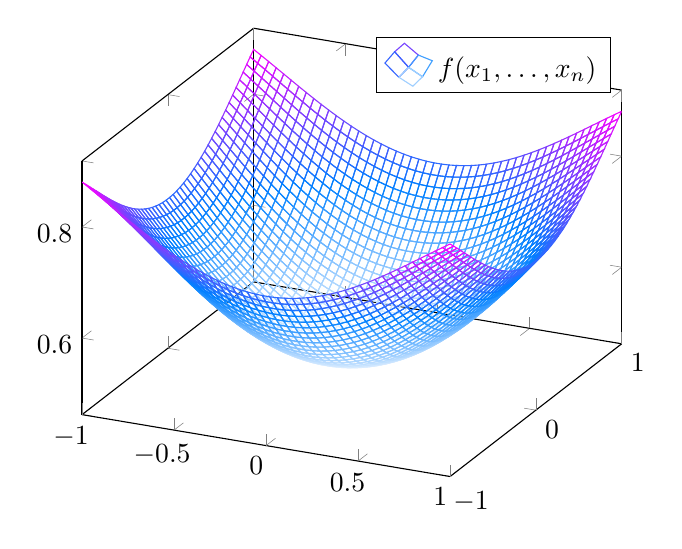
\begin{tikzpicture}
    \begin{axis}[
      % hide axis,
      colormap/cool,
      ]
      \addplot3[
      mesh,
      samples=50,
      domain=-1:1,
      ]
      {1/(1+exp(-(x^2+y^2)))};
      \addlegendentry{$f(x_1,\ldots,x_n)$}
    \end{axis}
  \end{tikzpicture}

  \caption{Visualisierung des Gradientenabstiegs}
\end{figure}

Waehrend des Gradientenverfahren konvergiert der Punkt $\vec{p}_t$ zu einem belibigen \textit{lokalen} Minimum, abhängig davon wie der Startpunkt $\vec{p}_0$ gewaehlt wurde.
Da dieser meist zufaellig bestimmt wird, ist es eine Glückssache ein sehr niedriges Minimum zu finden.
\para{}
Die sogennante \keyword{Lernrate} $\eta$ aus Gleichung (\ref{eq:gradientdescent}) ist ein Hyperparameter.
Sie ist ein positiver Proportionalitatsfaktor, welcher die Schrittgroesse des Gradientenabstieg bestimmt. Sie muss je nach zu minimierender Funktion anderst gewaehlt werden.
Dabei hilft nur ausporbieren. Falls $\eta$ nicht gut gewahelt wurde, gibt es Probleme beim Training:
\begin{itemize}
\item{Falls $\eta$ zu klein ist, verlaueft das Trainings unnotig langsam und braucht sehr lange.
    Ausserdem kann es passieren, dass man bei einem hohen lokalen Minimum stecken bleibt.}

\item{Falls $\eta$ zu gross ist, passiert es, dass man ueber das lokale Minimum hinaus schiesst und nur darum herum springt.}
\end{itemize}

\begin{figure}[h!]
  \centering
  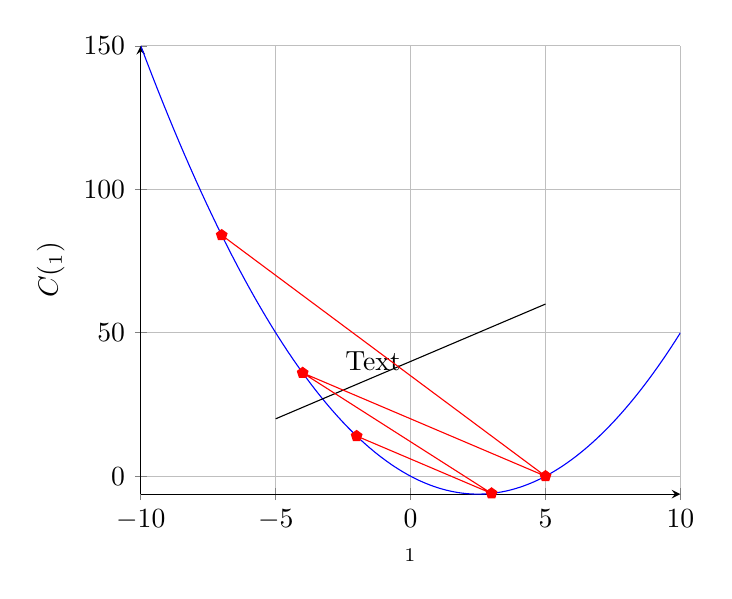
\begin{tikzpicture}
    \begin{axis}[
      axis lines = left,
      xlabel = $\param_1$,
      ylabel= {$C(\param_1)$},
      grid=major,
      ]
      \addplot [
      domain=-10:10,
      samples=100,
      color=blue
      ]
      {x^2 - 5*x};

      \draw (axis cs:-5,20) -- node[left]{Text} (axis cs:5,60);
      \addplot[color=red,mark=pentagon*,samples at={-7,5,-4,3,-2}] {x^2 - 5*x};

      \pgfmathparse{sin(60)}\pgfmathresult

    \end{axis}
  \end{tikzpicture}
  \caption{Visualisierung verschiedener Lernraten}
\end{figure}




\subsection{Stochastisches Gradientenverfahren fuer Machine Learning}
Wie vorhin erklaert, wird fuer das Trainieren eines Modells das Gradientenverfahren benutzt.
Konkret wird die Kostenfunktion $C(\vec{y},\vec{\hat{y}}\ |\ \param_0,\ldots,\param_n)$
($\param$ sind die Modellparameter, $\vec{y}$ die Vorhersagen und $\vec{\hat{y}}$
die Labels) minimieren, indem die Parameter angepasst werden. Dadurch macht das Modell immer bessere Vorhersagen.
Fuer nur eine Iteration des Gradientenverfahren, muesste man den Gradienten fuer den
\textit{gesamten} Trainingsdatensatz berechnen.
Dies waere zwar ein exakter Prozess, aber ein extrem langsamer zugleich.
Bei grossen Datensaetzen wuerde es eine Ewigkeit dauern, bis das Modell nur annahernd guete Vorhersagen machen wuerde.
\para{}
Aus diesem Grund verwendet man eine leicht abgeänderte Variante dieses
Verfahren, naemlich das \keyword{Stochastische Gradientenverfahren} (engl.:
Stochastic Gradient Descent) (SGD).
Hierfuer wird der ``echte'' Gradient des gesamten Datensatzes mit dem Gradienten einiger Trainingsbeispiel approximiert.
Dazu wird der Trainingsdatensatz in sogennante \keyword{Mini-Batches} eingeteilt und der Gradient jeweils pro Mini-Batch berechnet.
Als Konsequenz finden deutlich mehr Iterationen statt in \textit{einer}
Durchkaemmung der Trainingsdaten, welche man als \keyword{Epoche} bezeichnet. Oft wird mehrere Epochen lang trainiert.
Der Gradient eines genug grossen Mini-Batches ist zwar nicht ganz exakt, aber approximiert den Gradieten des gesamten Datensatzen genuegend gut.
Sowohl die Mini-Batch Groesse, wie auch die Anzahl Epochen sind weitere Hyperparameter.
\para{}
Die partiellen Ableitungen der gesamten Trainingsdaten wird mit dem arithmetischen Mittel der partiellen Ableitungen eines Mini-Batches der Groesse $q$ approximiert. Siehe Gleichung (\ref{eq:minibatch_deriv}).
\begin{equation}\label{eq:minibatch_deriv}
  \partderiv{\bar{C}}{\param_k} \approx \frac{1}{q}\sum_{i=1}^{q} \partderiv{C_i}{\param_k}
\end{equation}

Eine Iteration des Stochastischen Graidentenverfahren wird analog zu Gleichung (\ref{eq:gradientdescent}) folgendermassen durchgefuehrt:
\begin{equation}\label{eq:sgd}
  \param_{k,t+1} = \param_{k,t} - \frac{\eta}{q} \sum_{i=1}^{q} \partderiv{C_i}{\param_{k,t}}
\end{equation}


\subsection{Adam Optimizer}
ZUSAMMENFASSUNG TRAININGSALGORITHMUS

\section{Trainingsphaenomene}

\subsection{Overfitting}

\pagebreak
\chapter{Deep Learning und Künstliche Neuronale Netze}
Das wohl beste Modell fuer die meisten Problemstellungen in Bereich Machinelles Lernen (Bilderkennung, Spracherkennung, etc.) ist das \keyword{Kuenstliche Neuronale Netz}, kurz KNN (eng.: Neural Network).
Die Methoden welche benutzt werden um Neuronale Netze zu traniert fasst man unter dem Begriff \keyword{Deep Learning} zusammen.

Kuenstliche Neuronale Netze sind zum Teil biologisch inspiriert von Nervensystemen von Lebewesen. Sie sind aber lediglich eine Abstraktion der Informationverarbeitung und versuchen nicht eine moeglichst genaue biologische Abbildung darzustellen.
Es gibt nicht nur eine Art von Neuralem Netz, sondern es exisitieren die
verschiedensten Architekturen, welche je nach Problemstellung ausgewaehlt werden
muessen. Diese Arbeit wird sich spaeter vorallem mit sogennanten Autoencodern auseinandersetzen.


\section{Perzeptron}
Um den Aufbau und die Funktion eines Kuenstlichen Neuronalen Netz besser zu
verstehen, wird im folgenden ein Vorgaenger des KNN erklaert: das \keyword{Perzeptron}.
\para{}
Das einlagige Perzeptron wurde erstmals 1958 von Frank Rosenblatt vorgestellt. Dieses
besteht aus einem einzigen Kuenstlichen Neuron. Dieses Kuenstliche Neuron
hat mehrere binaere Inputs und einen einzigen binaeren Output. Binaer
bedeutet, dass der Wert nur entweder 0 (\textit{aus}) oder 1 (\textit{ein}) sein
kann. Des weiteren besitzt es mehrere sogenannte \keyword{Gewichte} $w_1, \ldots,
w_n \in \set{R}$, fuer jeden Input ein Gewicht.
Diese sind reelle Zahlen, welche das Verhalten des Perzeptron bestimmen.
Die \keyword{gewichtete Summe}, also die Summe aller Produkte der Inputs mit
ihrem Gewicht, wird mit $\tilde{z}$ bezeichnet.
Sie ist das gleiche wie das Skalarprodukt des Gewichtevektor mit dem Inputvektor:
\begin{equation*}
  \tilde{z} = \sum_{i=1}^{n} w_i x_i = \vec{w} \cdot \vec{x}
\end{equation*}
\para{}
Zusaetzlich besitzt das Perzeptron einen \keyword{Schwellenwert} $\tilde{b}$.
Zusammen mit den Gewichten, bildet er die Modellparameter.
Das Perzeptron verhaelt sich so, dass falls die gewichtete Summe groesser als der
Schwellwert ist, das Neuron feuert, d.h.\ der Output betraegt 1. Andernfalls ist er 0.
Siehe erster Teil der Gleichung (\ref{eq:perzeptron_1}).
Es ist gaengig die Ungleichung der Bedingung in die Nullstellenform zu bringen
und $\tilde{b}$ durch die \keyword{Neigung} (engl.: Bias)
$b = -\tilde{b}$ zu ersetzten. Somit lautet die Ungleichung: $\tilde{z} + b
> 0$. Der Term $\tilde{z} + b$ wird mit $z$ bezeichnet. Siehe Rest der Gleichung (\ref{eq:perzeptron_1}).
Die Neigung gibt an wie stark das Neuron dazu neigt zu feuern. Ein hohes $b$
laesst ein Neuron auch trotz einigen Nullen in den Inputs feuern, waehrend es
fuer ein tiefes $b$ nicht feuern lassen wuerde.

\begin{equation}\label{eq:perzeptron_1}
  p(\vec{x}) =
  \begin{cases}
    1 & \quad \text{falls } \tilde{z} > \tilde{b}\\
    0 & \quad \text{ansonsten}
  \end{cases}
  \quad =
  \begin{cases}
    1 & \quad \text{falls } \tilde{z} + b > 0\\
    0 & \quad \text{ansonsten}
  \end{cases}
  \quad =
  \begin{cases}
    1 & \quad\text{falls } \vec{w} \cdot \vec{x} + b > 0\\
    0 & \quad\text{ansonsten}
  \end{cases}
\end{equation}

\begin{figure}[h!]
  \centering
  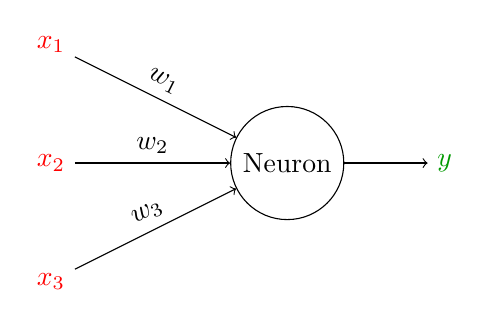
\begin{tikzpicture}
    \path (3,0) node [circle,draw](neuron){Neuron};
    \path[red] (0,1.5) node(x1){$x_1$} (0,0) node(x2){$x_2$} (0,-1.5) node(x3){$x_3$};
    \path[black!40!green] (5,0) node(y1){$y$};
    \draw[->] (x1) -- node[above,sloped]{$w_1$} (neuron);
    \draw[->] (x2) -- node[above,sloped]{$w_2$} (neuron);
    \draw[->] (x3) -- node[above,sloped]{$w_3$} (neuron);
    \draw[->] (neuron) -- (y1);
  \end{tikzpicture}
  \caption{Perzeptron mit drei Inputs}
  \label{fi:perzeptron}
\end{figure}

Fuer das Trainieren des Perzeptron existieren spezielle Verfahren, welche hier
aber nicht relevant sind. Das Gradientenverfahren kann naemlich nicht verwendet
werden. Der Grund dafuer sollte spaeter in Sektion (\ref{sec:kuenstlicheNeuronen}) einleuchtend werden.

\subsection{Was kann ein Perzeptron erlernen?}
Nun stellt sich die Frage, was ein Perzeptron erlernen kann und wofuer es genutzt werden kann.
Das Perzeptron ist lediglich ein \keyword{Linearer Klassifikator} der Form
$y = w_1x_1 + \cdots + w_n x_n$.
Es kann die Features in zwei Klassen 0 oder 1 einordnen.
Ueberschreitet $y$ den Schwellenwert, werden die Features der Klasse 1 zugeordnet, sonst
der Klasse 0.
Jedoch muessen diese Klassen linear separierbar sein.
Das bedeutet, dass die Featurevektoren $\vec{x}$ durch eine Hyperebene trennbar
sein muessen.
Bei zwei Features (zwei Inputs) handelt es sich bei der Hyperebene um eine
Gerade welche die Vektoren auftrennt. Siehe Abbildung (\ref{fig:linearer_Klassifikator}).
Fuer drei Featuers ist es eine Ebene.
ZU ABSTRAKT -> BEISPIEL

Eine Funktionen, welche nicht linear separierbar ist (z.B\ XOR-Verknuepfungen),
kann von einem Perzeptron nicht erlernt werden.

\begin{figure}[h!]

  \caption{erfolgreiche lineare Separierung (links) und das Versagen bei XOR (rechts)}
  \label{fig:linearer_Klassifikator}
\end{figure}

\cite{wiki:perzeptron}

\subsection{Biologische Analogie}
SCHREIBEN
% Gewicht entscheidet ob inhibitorisch oder exaktorisch.
% Schwellenwert: Das Addieren eines Schwellenwerts  zur Netzeingabe verschiebt die gewichteten Eingaben. Die Bezeichnung bestimmt sich aus der Verwendung einer Schwellenwertfunktion als Aktivierungsfunktion, bei der das Neuron aktiviert wird, wenn der Schwellenwert überschritten ist. Die biologische Motivierung dabei ist das Schwellenpotential bei Nervenzellen. Mathematisch gesehen wird die Trennebene, die den Merkmalsraum auftrennt, durch einen Schwellenwert mit einer Translation verschoben.

% Hebbsche Lernregel

\begin{figure}[h!]

  \caption{Nervenzelle}
\end{figure}


\section{Erweiterung der Kuenstlichen Neuronen}\label{sec:kuenstlicheNeuronen}
Ein Perzeptron ist, wie vorhin erklaert, nur in der Lage, lineare Klassifikationen
durchzufuehren. Um nun auch kompliziertere Probleme zu loesen, muss das Prinzip
ausgebaut werden. Ausserdem brauchen wir ein Kuenstliches Neuron, welches sich
besonders gut als Baustein fuer KNNs eignet.

\subsection{Kuenstliche Neuronen im Allgemeinen}
Kuenstliche Neuronen sind immer so aufgebaut, dass sie einen oder mehrere Inputs
haben und einen einzigen Output. Zu jedem Input $x_i$ ist ein Gewicht
$w_{ji}$ assoziert. Zuerst wird die gewichtete Summe der Inputs $\tilde{z}$ gebildet.
Die Neigung $b$ wird ebenfalls draufaddiert, um $z$ zu erhalten. Nun muss
die sogennante Aktivierung $a$ gebildet werden. Sie entspricht dem Output des Neurons.
Die Aktivierung $a$ ist das Resultat der Aktivierungsfunktion $\varphi$ angewendet
auf $z$. $a = \varphi(z)$. Die verschiedenen Kuenstlichen Neuronen unterscheiden
sich fast nur in ihrer Aktivierungsfunktion.

\begin{figure}[h!]

  \caption{ein kuenstliches Neuron und seine Bestandteile}
\end{figure}

\subsection{Perzeptronen als Kuenstliche Neuronen}
Zuerst noch einmal ein Blick auf das Perzeptron im Angesicht der Aktivierungsfunktion.
Ein wesentlicher Unterschied des Perzeptron gegenueber sonstigen Kuenstlichen
Neuronen, besteht darin, dass seine Inputs und Outputs nur binaere Werte
annehmen koennen. Um dieses Verhalten des Perzeptron zu erhalten,
muss eine Stufenfunktion als Aktivierungfunktion verwendet werden: die Heaviside-Funktion $\Theta$.
Sie hat einen einzigen Stufensprung bei $x=0$ vom Wert 0 auf 1. Siehe Abb. (\ref{fig:heaviside}).

\begin{figure}[h!]
  \begin{minipage}[h!]{0.5\textwidth}
    \begin{equation*}
      \varphi^{\text{hlim}}(z) = \Theta(z) =
      \begin{cases}
        1 & \quad \text{falls } z \geq 0\\
        0 & \quad \text{falls } z < 0
      \end{cases}
    \end{equation*}

  \end{minipage}
  \begin{minipage}[h!]{0.5\textwidth}
    \centering
    \begin{tikzpicture}[scale=2.5]

      \draw[->] (-1.5,0) -- (1.5,0) node[right] {$x$}; % x-axes
      \draw[->] (0,-0.2) -- (0,1.2) node [above] {$y$}; % y-axes
      \draw[style=help lines,step=0.5] (-1.4,0) grid (1.4, 1.1);

      \foreach \x in {-1,-0.5,0.5,1}
      \draw[shift={(\x,0)}] (0pt,2pt) -- (0pt,-2pt) node[below,fill=bgcolor] {$\x$};

      \foreach \y in {0.5,1}
      \draw[shift={(0,\y)}] (2pt,0pt) -- (-2pt,0pt) node[left,fill=bgcolor] {$\y$};

      \draw[shift={(0,0)}] (0pt,0pt) node[below left,fill=bgcolor] {$O$};

      \draw[red,ultra thick] (-1.5,0) -- (0,0); % 0-red
      \draw[red,ultra thick] (0,1) -- (1.5,1); % 1-red
      \draw[red,ultra thick,dashed] (0,0) -- (0,1); % y-red
      \draw[draw=red,fill=white] (0,0) circle (0.05);
      \draw[draw=red,fill=red] (0,1) circle (0.05);

    \end{tikzpicture}
  \end{minipage}

  \caption{Definition und Graph der Heaviside-Funktion $\Theta$}
  \label{fig:heaviside}
\end{figure}

\subsection{Stueckweise lineare Neuronen}
Der naechste Schritt nach dem binaeren Perzeptron sind sogenannte stueckweise
lineare Neuronen.
Sie verwenden eine stueckweise lineare Aktivierungsfunktion. Diese bildet ein
beschraenktes Intervall linear ab. Die Werte ausserhalb werden auf die
konstanten Werte 0 oder 1 abbgebildet. Siehe Abb. (\ref{fig:stueckweiselinear}).
\para{}
Die Inputs koennen jetzt beliebige reelle Zahlen sein (vorzugsweise in der Naehe
von 0 und 1).
Ein KNN aus ausschliesslich linearen Neuronen ist ziemlich nutzlos, da jedliche Verkettung von
linearen Funktion auch durch eine einzige lineare Funktion dargestellt werden
koennte. Somit hat ein KNN gegenueber einem einzelnen Neuron keinen Mehrwert.
Ausserdem koennen mit diesen Neuron auch nur lineare Probleme geloest werden.

\begin{figure}[h!]
  \begin{minipage}[h!]{0.5\textwidth}
    \begin{equation*}
      \varphi^{\text{pwl}}(z) =
      \begin{cases}
        1 & \quad \text{falls } z > \frac{1}{2}\\
        z + \frac{1}{2} & \quad \text{falls } -\frac{1}{2} < z < \frac{1}{2}\\
        0 & \quad \text{falls } z < \frac{1}{2}
      \end{cases}
    \end{equation*}

  \end{minipage}
  \begin{minipage}[h!]{0.5\textwidth}
    \centering
    \begin{tikzpicture}[scale=2.5]

      \draw[->] (-1.5,0) -- (1.5,0) node[right] {$x$}; % x-axes
      \draw[->] (0,-0.2) -- (0,1.2) node [above] {$y$}; % y-axes
      \draw[style=help lines,step=0.5] (-1.4,0) grid (1.4, 1.1);

      \foreach \x in {-1,-0.5,0.5,1}
      \draw[shift={(\x,0)}] (0pt,2pt) -- (0pt,-2pt) node[below,fill=bgcolor] {$\x$};

      \foreach \y in {0.5,1}
      \draw[shift={(0,\y)}] (2pt,0pt) -- (-2pt,0pt) node[left,fill=bgcolor] {$\y$};

      \draw[shift={(0,0)}] (0pt,0pt) node[below left,fill=bgcolor] {$O$};

      \draw[red,ultra thick] (-1.5,0) -- (-0.5,0); % 0-red
      \draw[red,ultra thick] (0.5,1) -- (1.5,1); % 1-red
      \draw[red,ultra thick] (-0.5,0) -- (0.5,1); % d-red

      \draw[draw=red,fill=red] (-0.5,0) circle (0.03);
      \draw[draw=red,fill=red] (0.5,1) circle (0.03);


    \end{tikzpicture}
  \end{minipage}

  \caption{Formel und Graph einer stueckweisen linearen Funktion}
  \label{fig:stueckweiselinear}
\end{figure}


\subsection{Sigmoide Neuronen}
Die logische naechste Erweiterung sind nicht-lineare Neuronen.
Ein sehr beliebter Kandidat dafuer sind Sigmoide Neuronen.
Den Namen haben sie von ihrer Aktivierungsfunktion: der Sigmoidfunktion $\sigma$.
Eine sehr wichtige Eigenschaft von ihr ist, dass sie - im Gegensatz zu den vorhin
genannten Aktivierungsfunktion - ueberall differenzierbar und strikt monoton
steigend ist. Erst fuer diese Aktivierungsfunktion, kann das Gradientenverfahren
angewendet werden und somit das KNN trainiert werden. Die anderen
Funktionen haben Stellen bei welchen die Ableitungsfunktion null
betraegt, somit kann das lokale Minimum nicht gefunden werden.
Nicht nur die Sigmoidfunktion erfuellt diese Bedingungen, sondern auch andere. Die Sigmoidfunktion wird
bevorzugt, da ihre Ableitung sehr simpel ist, siehe Abb. (\ref{fig:sigmoid}).
Die Nicht-linearitaet dieser Neuronen ermoeglicht ein Erlernen von deutlich komplexeren Sachverhalten.
Und wie spaeter in Sektion (\ref{sec:UAT}) erlautert, ist es moeglich mit der Kompostion von nicht-linearen
Funktionen jede belibige Funktion zu approximieren!
\para{}
Die Sigmoid-Funktion besitzt eine einzige Wendestelle $\sigma''(x=0)=0$ und hat
zwei Asymptoten, eine $\ds\lim_{x \to -\infty} \sigma(x)=0$
und eine zweite $\ds\lim_{x \to \infty} \sigma(x)=1$. Siehe Abb. (\ref{fig:sigmoid}).


\begin{figure}[h!]
  \begin{minipage}[h!]{0.5\textwidth}
    \begin{align*}
      \varphi^{\text{sig}}(z) &= \sigma(z) = \frac{1}{1 + e^{-z}}\\
      \sigma'(z)&=\sigma(z)(1-\sigma(z))
    \end{align*}
  \end{minipage}
  \begin{minipage}[h!]{0.5\textwidth}
    \centering
    \begin{tikzpicture}[scale=2.5]

      \draw[->] (-1.5,0) -- (1.5,0) node[right] {$x$}; % x-axes
      \draw[->] (0,-0.2) -- (0,1.2) node [above] {$y$}; % y-axes
      \draw[style=help lines,ystep=0.5,xstep=0.25] (-1.4,0) grid (1.4, 1.1);

      \foreach \x/\xtext in {-1/-4,-0.5/-2,0.5/2,1/4}
      \draw[shift={(\x,0)}] (0pt,2pt) -- (0pt,-2pt) node[below,fill=bgcolor] {$\xtext$};

      \foreach \y in {0.5,1}
      \draw[shift={(0,\y)}] (2pt,0pt) -- (-2pt,0pt) node[left,fill=bgcolor] {$\y$};

      \draw[shift={(0,0)}] (0pt,0pt) node[below left,fill=bgcolor] {$O$};


      \draw[red,ultra thick,x=0.25cm] plot[domain=-6.0:6.0] (\x,{1/(1+exp(-\x)) });

    \end{tikzpicture}
  \end{minipage}

  \caption{Definition, Ableitung und Graph der Sigmoid-Funktion $\sigma$}
  \label{fig:sigmoid}
\end{figure}




\section{Topologie der Kuenstlichen Neuronalen Netzen}
Nun sollten diese Sigmoiden-Neuronen als Bausteine verwendet werden, um ein Kuenstliches
Neuronales Netz zu bilden. Dazu werden sie miteinander verbundet und bilden so ein Netz,
aehnlich wie ein Nervensystem.
Diese Neuronen sind in verschieden Schichten (engl.: Layers)
arangiert. Die erste ist die \keyword{Inputschicht}. Sie behinhalten die
Inputneuronen. Dies sind eigentlich keine richtigen
Neuronen sondern eher Platzhalter fuer ihren jeweiliges Feature $x_i$. Als letztes kommt die
\keyword{Outputschicht} mit den Outputneuronen, welche jeweils einen Outputwert $y_i$
besitzen. Dazwischen liegen die \keyword{Zwischenschichten} (engl.: Hiddenlayer). Von ihnen kann es
beliebig viele geben und in ihnen beliebig viele Neuronen.
Falls viele Zwischenschichten verwendet werden, bezeichnet man das Netzwerk als
``deep''. Daher ruert auch der Name des Deep Learnings.
Der Aufbau eines KNN bezeichnet man als \keyword{Topologie} des Netzes. Die
Topologie umfasst viele Hyperparameter. Darunter sind zum Beispiel die Anzahl Zwischenschichten, wie auch
die Anzahl Neuronen pro Schicht.
\para{}
Jedes Neuron aus einer Schicht ist mit jedem Neuron aus der naechsten Schicht ueber
Verbindungen gekoppelt. Alle Verbindungen besitzten ein Gewicht analog zu den Inputs des
Perzeptron. Die Aktivierung, also der Output, eines Neurons wandert entlang den jeweiligen
Verbindung zu allen Neuronen der naechsten Schicht und dient als deren Input.
Die soeben beschriebe Art von KNN nennt man \keyword{Feedforward-Netz}, da alle Werte
ausschliesslich nach vorne propagiert werden.
\para{}
In Abbildung (\ref{fig:nn_layers}) ist ein Beispiel eines Neuronalen Netzes
abgebildet. In diesem Fall besitz es sowohl 4 Inputs, wie auch 4 Outputs. Es hat
ausserdem 3 Zwischenschichten. Die zwei aueserren Zwischenschichten haben 3 Neuronen und die dazwischen
hat sogar 4 Neuronen.
\para{}
Die Hoffnung beim Trainieren von KNNs besteht darin, dass das Modell fuer jede
weiter Schicht eine hoeheres Abstraktionsniveau erreicht. Wuerde man zum
Beispiel ein Netzwerk zur Gesichtserkennung trainieren, koennte man sich den
Erkennungsprozess folgendermassen vorstellen. Die erste Zwischenschicht erkennt
Kanten und Konturen. Die zweite vereint diese Merkmale zu Ecken und primitive
geometrische Formen. Die dritte Schicht sollte dann schon komplexere
geometrische Formen erkennen, welche gewissen Gesichtmerkmalen, wie der Nase, aehneln. Die letzten Schichten sollte dann all diese
Merkmale zusammensetzen und so ein Gesicht erkennen.

SCHICHTENBESCHRIFTUNG HINZUFUEGEN; BIAS ALS EIGENES NEURON?
\begin{figure}[h!]
  \centering
  \begin{tikzpicture}[>=latex]

    \tikzstyle{netstyle} = [matrix of nodes,nodes={draw,circle,inner sep=0, minimum size=1cm},column sep=0.5cm,row sep=-9pt]
    \tikzstyle{cl} = [draw=none,fill=none]
    \tikzstyle{heading} = [clear,text width=15mm,text centered]
    \tikzstyle{inp} = [fill=red!70!bgcolor]
    \tikzstyle{hid} = [fill=blue!70!bgcolor]
    \tikzstyle{ou} = [fill=green!70!bgcolor]

    \matrix[netstyle] (mat)
    {
      |[inp]| $x_1$     & |[cl]| & |[cl]| & |[hid]|$h_1^2$ & |[cl]| & |[cl]| & |[ou]|$y_1$ \\
      |[cl]| & |[cl]| & |[hid]|$h_1^1$   & |[cl]| & |[hid]|$h_1^3$ & |[cl]| & |[cl]| \\
      |[inp]| $x_2$     & |[cl]| & |[cl]| & |[hid]|$h_2^2$ & |[cl]| & |[cl]| & |[ou]|$y_2$ \\
      |[cl]| & |[cl]| & |[hid]|$h_2^1$   & |[cl]| & |[hid]|$h_2^3$ & |[cl]| & |[cl]| \\
      |[inp]| $x_3$     & |[cl]| & |[cl]| & |[hid]|$h_3^2$ & |[cl]| & |[cl]| & |[ou]|$y_3$ \\
      |[cl]| & |[cl]| & |[hid]|$h_3^1$   & |[cl]| & |[hid]|$h_3^3$ & |[cl]| & |[cl]| \\
      |[inp]| $x_4$     & |[cl]| & |[cl]| & |[hid]|$h_4^2$ & |[cl]| & |[cl]| & |[ou]|$y_4$ \\
    };

    % titels
    \node [yshift=1cm] at (mat-1-1) {Inputschicht};
    \node [yshift=1cm] at (mat-1-4) {Zwischenschichten};
    \node [yshift=1cm] at (mat-1-7) {Outputschicht};

    % dots
    % \node [yshift=-1cm,scale=2] at (mat-7-1) {$\vdots$}; % for inputs
    % \node [yshift=-1cm,scale=2] at (mat-6-3) {$\vdots$};
    % \node [yshift=-1cm,scale=2] at (mat-7-4) {$\vdots$};
    % \node [yshift=-1cm,scale=2] at (mat-6-5) {$\vdots$};
    % \node [yshift=-1cm,scale=2] at (mat-7-7) {$\vdots$}; % for outputs

    % input -> hidden1
    \foreach \ai in {1,3,...,7} {
      \foreach \aii in {2,4,6}
      \draw[->] (mat-\ai-1) -- (mat-\aii-3);
    }

    % hidden1 -> hidden2
    \foreach \ai in {2,4,...,6} {
      \foreach \aii in {1,3,...,7}
      \draw[->] (mat-\ai-3) -- (mat-\aii-4);
    }

    % hidden2 -> hidden3
    \foreach \ai in {1,3,...,7} {
      \foreach \aii in {2,4,6}
      \draw[->] (mat-\ai-4) -- (mat-\aii-5);
    }

    % hidden3 -> output
    \foreach \ai in {2,4,...,6} {
      \foreach \aii in {1,3,...,7}
      \draw[->] (mat-\ai-5) -- (mat-\aii-7);
    }

  \end{tikzpicture}
  \caption{Schichten eines KNNs}
  \label{fig:nn_layers}
\end{figure}

\section{Vorwaertspropagierung}
Jetzt, da der Aufbau eines KNNs erklaert wurde, sollte nun die mathematische Funktionsweise
des Modells erklaert werden. Hierfuer muessen einige Konventionen zur
Bezeichnung der Teile eines KNNs getroffen werden:

\begin{itemize}

\item{$n_j^l$ ist das $j$-te Neuron in der $l$-ten Schicht.}
\item{$z_j^l$ ist die gewichtete Summe der Inputs des $j$-ten Neuron in der $l$-ten Schicht.}
\item{$a_j^l$ ist die Aktivierung des $j$-ten Neurons in der $l$-ten Schicht.}
\item{$b_j^l$ ist die Neigung fuer das $j$-te Neuron in der ($l+1$)-ten Schicht ausgeht.
    \footnote{
      Diese Konvention wurde gewaehlt, damit die folgenden Gleichungen simpler sind.
    }
  }
\item{$w_{j,k}^l$ ist das Gewicht der Verbindung vom $k$-ten Neuron
    in der $l$-ten Schicht zum $j$-ten Neuron in der ($l+1$)-ten Schicht.
    \footnote{
      Man beachte die Reihenfolge!\\
      Diese Konvention scheint zwar auf den ersten Blick unintuitiv, macht jedoch
      Sinn fuer die spaeteren mathematischen Operationen mit Matrizen in Sektion
      (\ref{sec:backpropagation}).
    }}

\item{$L$ soll die gesamte Anzahl der Schichten sein.}

\item{$|l|$ ist die Anzahl Neuronen in der $l$-ten Schicht.
    \footnote{
      Diese Schreibweise hat nichts mit dem Betrag zu tun, sondern wird einfach
      gewaehlt, da sie sehr platzsparend ist.
    }
  }

\item{$\varphi$ ist die gewaehlte Aktivierungsfunktion (grundsaetzlich ist diese
    immer die Sigmoidfunktion $\sigma$).}

\end{itemize}

ABBILDUNG MIT NEURONBESTANTEILEN (GEWICHTEBESCHRIFTUNGEN UND NEIGUNGEN)

DIE GEWICHTBESCHRIFTUNGEN IN ABBILDUNG 11 sind falsch! Die Gewichtsindizes
beginnen mit 0 und ended mit L-1
\begin{figure}[h!]
  \centering
  \begin{tikzpicture}[>=latex]

    \tikzstyle{netstyle} = [matrix of nodes,nodes={draw,circle,inner sep=0, minimum size=1.25cm},column sep=0.5cm,row sep=-9pt]
    \tikzstyle{cl} = [draw=none,fill=none]
    \tikzstyle{sy} = [cl,font=\LARGE]
    \tikzstyle{heading} = [clear,text width=15mm,text centered]
    \tikzstyle{inp} = [fill=red!70!bgcolor]
    \tikzstyle{hid} = [fill=blue!70!bgcolor]
    \tikzstyle{ou} = [fill=green!70!bgcolor]

    \matrix[netstyle] (mat)
    {
      |[inp]|$a_1^0$     & |[cl]| & |[cl]| & |[cl]| & |[cl]| & |[cl]| & |[ou]|$a_1^L$ \\
      |[cl]| & |[cl]| & |[hid]|$a_1^1$   & |[sy]| $\cdots$ & |[hid]|$a_1^{L-1}$ & |[cl]| & |[cl]| \\
      |[inp]|$a_2^0$     & |[cl]| & |[cl]| & |[cl]| & |[cl]| & |[cl]| & |[ou]|$a_2^L$ \\
      |[cl]| & |[cl]| & |[hid]|$a_2^1$   & |[sy]| $\cdots$ & |[hid]|$a_2^{L-1}$ & |[cl]| & |[cl]| \\
      |[inp]|$a_3^0$     & |[cl]| & |[sy]| $\vdots$ & |[cl]| & |[sy]| $\vdots$ & |[cl]| & |[ou]|$a_3^L$ \\
      |[sy]| $\vdots$ & |[cl]| & |[hid]|$a_{|1|}^1$ & |[sy]|$\cdots$ & |[hid]|$a_{|L-1|}^{L-1}$ & |[cl]| & |[sy]| $\vdots$ \\
      |[inp]|$a_{|0|}^0$ & |[cl]| & |[cl]| & |[cl]| & |[cl]| & |[cl]| & |[ou]|$a_{|L|}^L$ \\
    };

    % titels
    \node [yshift=1.5cm] at (mat-1-1) {Inputschicht};
    \node [yshift=1.5cm] at (mat-2-4) {Zwischenschichten};
    \node [yshift=1.5cm] at (mat-1-7) {Outputschicht};

    % input -> hidden1
    \foreach \ai in {1,3,...,7} {
      \foreach \aii in {2,4,...,6}
      \draw[->] (mat-\ai-1) -- node[above,sloped]{} (mat-\aii-3);
    }

    % hidden1 ->...
    \foreach \ai in {2,4,...,6} {
      \foreach \aii in {2,4,...,6} {
        \node (A) at (mat-\ai-3) {};
        \node (B) at (mat-\aii-5) {};
        \draw[left color=black,right color=white] (mat-\ai-3) -- ($(A)!0.3!(B)$);
      }
    }

    % ...-> hidden2
    \foreach \ai in {2,4,...,6} {
      \foreach \aii in {2,4,...,6} {
        \node (A) at (mat-\ai-3) {};
        \node (B) at (mat-\aii-5) {};
        \draw[left color=black,right color=white] ($(A)!0.7!(B)$) -- (mat-\aii-5);
      }
    }

    % hidden3 -> output
    \foreach \ai in {2,4,...,6} {
      \foreach \aii in {1,3,...,7}
      \draw[->] (mat-\ai-5) -- node[above,sloped]{} (mat-\aii-7);
    }

  \end{tikzpicture}
  \label{fi:nn_layers}
  \caption{zum Verstaentniss der Nomenklatur}
\end{figure}

\begin{figure}[h!]

  \caption{Neuron mit Gewichtbeschriftungen und Neigung}
\end{figure}


\par\bigskip
Die Vorwaertspropagierung beginnt bei den Inputneuronen, welche jeweils
einen Inputwert in sich tragen. Diese werden, um fuer eine kohaerente Nomenklatur zu sorgen,
analog zu den Aktivierungen der anderen Neuronen mit $a_j^0$ bezeichnet, wobei
$j$ der Index des Neurons ist.\par
Nun muessen die restlichen Aktivierungen der Neuronen berechnet werden. Dies geschieht rekursiv, anhand der
Aktivierungen der voherigen Schicht. Und zwar folgendermassen (ersichtlich in
Gleichung (\ref{eq:gewichtete_summe_normal})): \\
Zuerst laueft eine Summe ueber alle Neuronen $n_k^{l}$ der jetztigen Schicht
$l$. Dabei wird die gewichtete Summe der Aktivierungen $a_k^{l}$ mit den
assozierten Gewichten $w_{j,k}^l$ gebildet. Hierbei ist das Gewicht jenes, welches das
$k$-te Neuron der $l$-ten Schicht mit dem $j$-ten Neuron der ($l+1$)-ten Schicht verbindet.
Zusaetzlich gehoert zu der gewichteten Summe auch die jeweilige Neigung $b_j^l$, welche
dazuaddiert wird. Diese gewichtete Summe wird mit $z_j^{l+1}$ bezeichnet.

\begin{equation}\label{eq:gewichtete_summe_normal}
  z_j^{l+1} = \sum_{k=1}^{N_l} w_{j,k}^l a_k^l + b_j^l
\end{equation}

Auf diese Summe wird dann die Aktivierungsfunktion $\varphi$ angewandt.
Das ist dann die Aktivierung $a_j^{l+1}$ des $j$-ten Neurons in der ($l+1$)-ten Schicht.

\begin{equation}\label{eq:aktivierung_normal}
  a_j^{l+1} = \varphi\left(\sum_{k=1}^{N_l} w_{j,k}^l a_k^{l} + b_j^l \right) = \varphi \left( z_j^{l+1} \right)
\end{equation}
\par\bigskip
Da KNNs weit verbreitet sind in der Bilderkennung und Spracherkennung, ist es
nicht unueblich, dass diese sehr viele Neuronen und Verbindungen (ueber 100'000) besitzen.
Um hierbei nicht den Ueberblick zu verlieren und um nicht in den Indizes zu
ertrinken, greift man auf \keyword{Lineare Algebra} zurueck. Man verwendet
Matrizen und Vektoren um die vielen Variabeln zusammenzufassen.
Ausserdem besteht ein weiterer Vorteil darin, dass Computer mithilfe von Vektor-
und Matrixoperationen die Berechnungen parallisieren koennen und in kuerzerer
Zeit und mit weniger Ressourcen viele Brechnungen gleichzeitig ausfuehren koennen.
Dies beschleunigt das Training der Modelle um
ein Vielfaches. Dies wird spaeter in Sektion
(\ref{sec:tensorflow}) noch weiter thematisiert.
\para{}
Die Inputs $\vec{x}$, Outputs $\vec{y}$ und Labels $\vec{\hat{y}}$ haben wir schon von Anfang an als Vektoren geschrieben.
Nun sollen noch die Parameter und die restlichen Komponenten eines KNNs als Vektoren und Matrizen geschrieben werden.
Sowohl alle gewichteten Summen $z_j^l$, wie auch alle Aktivierungen $a_j^l$
einer Schicht $l$, werden in Vektoren $\vec{z}^l$ und $\vec{a}^l$ zusammengefasst.
Alle Neigung $b_j^l$ fuer eine Schicht ($l+1$) bilden ebenfalls eines Vektor $\vec{b}^l$.
Zu guter letzt, wird noch eine \keyword{Gewichtsmatrix} $\mat{W}^l \in
\set{R}^{|l+1| \times |l|}$
definiert. Sie enthaltet alle Gewichte welche die $l$-te
Schicht \textit{zu} der ($l+1$)-ten Schicht verbindet.
Das heisst der Eintrag in der $j$-ten Zeile und in
der $k$-ten Spalte ist $w_{j,k}^l$ und verbindet so das Neuron $n_k^{l}$ zu
dem Neuron $n_j^{l+1}$.
\para{}

\begin{align*}
  \vec{z}^l &=  \trans{\begin{pmatrix} z_1^l & z_2^l & \cdots & z_{|l|}^l \end{pmatrix}} \\
  \vec{a}^l &=  \trans{\begin{pmatrix} a_1^l & a_2^l & \cdots & a_{|l|}^l \end{pmatrix}} \\
  \vec{b}^l &=  \trans{\begin{pmatrix} b_1^l & b_2^l & \cdots & b_{|l+1|}^l \end{pmatrix}} \\
\end{align*}
\begin{equation*}
  \mat{W}^l =
  \begin{pmatrix}
    w_{1,1}^l & w_{1,2}^l & \cdots & w_{1,|l|}^l \\[0.3em]
    w_{2,1}^l & w_{2,2}^l & \cdots & w_{2,|l|}^l \\[0.3em]
    \vdots & \vdots & \ddots & \vdots \\[0.3em]
    w_{|l+1|,1}^l & w_{|l+1|,2}^l & \cdots & w_{|l+1|,|l|}^l
  \end{pmatrix}
\end{equation*}

\para{}
Mit diesen Definitionen kann nun Gleichung (\ref{eq:gewichtete_summe_normal}) in
Matrixform geschrieben werden, denn die Matrixmultiplikation von $\mat{W}^l$ mit
$\vec{a}^{l}$ ergibt einen Vektor $\vec{\tilde{z}}^{l+1}$, welcher alle gewichteten
Summen $\tilde{z}_j^{l+1}$ ohne die jeweilige Neigung enthaelt.

STIMMT DIESE GLEICHUNG? (GLAUBE SCHON)
\begin{equation*}
  \mat{W}^l \vec{a}^{l} = \trans{\begin{pmatrix}\ds \sum_{i=1}^{|l|} w_{i,1}^l a_i^l &\ds \sum_{i=1}^{|l|} w_{i,2}^l a_i^l & \cdots &\ds \sum_{i=1}^{|l|} w_{i,|l+1|} a_i^l \end{pmatrix}} = \vec{\tilde{z}}^{l+1}
\end{equation*}
\para{}

Nun muessen wir noch den Neigungsvektor $\vec{b}^l$ draufaddieren und wir
erhalten Gleichung (\ref{eq:gewichtete_summe_matrix}), mithilfe dessen wir den
Vektor der gewichteten Summen $\vec{z}^{l+1}$ bilden koennen.

\begin{equation}\label{eq:gewichtete_summe_matrix}
  \vec{z}^{l+1} = \mathbf{W}^{l} \vec{a}^{l} + \vec{b}^{l}
\end{equation}
\para{}
Der letzte Schritt besteht noch darin die Aktivierungsfunktion auf $\vec{z}^{l+1}$
anzuwenden um den Aktivierungsvektor $\vec{a}^{l+1}$ zu bilden.
Hierfuer muss aber noch ein neues mathematisches
Konzept eingefuehrt werden: die Vektorisierung einer Funktion.
\para{}

\begin{defbox}{Vektorisierung einer Funktion}
  Die Vektorisierung einer Funktion $f$, geschrieben als $\vecf{f}[\vec{v}]$ ist eine
  neue Funktion, welche als Rueckgabewert einen Vektor hat, auf dessen
  Komponenten jeweils immer die Funktion $f$ angewendet wird.
  \begin{equation*}
    \vecf{f}[\vec{v}]=
    \begin{pmatrix}
      f(v_1)\\
      \vdots \\
      f(v_n)\\
    \end{pmatrix}
  \end{equation*}
\end{defbox}
\para{}

Nun kann ganz einfach die vektorisierte Aktivierungsfunktion $\vecf{\varphi}$ auf
$\vec{z}^{l+1}$ angewandt werden.

\begin{equation}\label{eq:aktivierung_matrix}
  \vec{a}^{l+1} = \vecf{\varphi} \left[\mat{W}^{l} \vec{a}^{l} + \vec{b}^{l} \right] = \vecf{\varphi} \left[ \vec{z}^{l+1} \right]
\end{equation}

\para{}
\cite{Nielsen}

\subsection{Modellparameter initalisieren}
Ein Schritt der getan werden muss, bevor das Training beginnt, ist das
Initalisieren aller Modellparameter, in diesem Fall die Gewichte und Neigungen.
Dies ist ein sehr essentieller Schritt, denn diese Startwerte entscheiden
erheblich ueber die Leistungsfaehigkeit des Modells.
\para{}
Wie in Sektion (\ref{sec:gradientenverfahren}) gezeigt, muss am Anfang des
Gradientenverfahrens ein Startpunkt $\vec{p}_0$ innerhalb des Gradientenfeldes
$\vecf{\nabla}$ gewaehlt werden, von welchem aus der Gradientenabstieg beginnt.
Da wir das Gradientenverfahren zur Optimierung der Modellparameter verwenden,
ist unser Startpunkt, der Vektor aller Hyperparameter
$\vec{\param} = \trans{\begin{pmatrix} \param_1 & \cdots & \param_n \end{pmatrix}}$.
Dieser Startpunkt entscheidet darueber, in welches lokale Minimum konvergiert
wird und bestimmt somit auch die bestmoegliche Exaktheit der Vorhersagen. Falls
schlecht Initalwerte gewaehlt werden, konvergiert der Punkt in ein hohes lokales
Minimum, was grosse Kostenfunktionswerte und schlecht Vorhersagen verursacht.
\para{}
Es ist nicht moeglich im Vorhinein zu wissen, welche Initalwerte gute Resultate
liefern. Man muss ausprobieren, deshalb initalisert man gaengierweise die
Hyperparameter mit Zufallswerten. Dafuer nimmt man aber nicht irgendwelche
Zufallsvariablen sondern man benutzt die Gauss'sche Normalverteilung
$\mathcal{N}(\mu,\sigma^2)$ bzw. ihre Dichtefunktion
\[\ds \phi(x\ |\ \mu,\sigma^2) = \frac{1}{\sqrt{2\pi\sigma^2}} \text{exp} \left\{-\frac{{(x-\mu)}^2}{2\sigma^2}\right\} \]
\para{}


% \pgfplotsset{compat=1.15}
% \pgfmathdeclarefunction{gauss}{2}{%
% \pgfmathparse{1/(#2*sqrt(2*pi))*exp(-((x-#1)^2)/(2*#2^2))}%
% }
%   \usetikzlibrary{arrows.meta}    % <--- added

\begin{figure}[h!]
  \centering
  % \begin{tikzpicture}[
  %   every pin/.style = {pin edge={Latex-,thin,black}}
  %   ]
  %   \begin{axis}[
  %     width=15cm,height=6cm,
  %     scale only axis,
  %     axis lines=middle,
  %     ymin=0,ymax=0.45,
  %     axis line style = thick,
  %     xtick={-3,-2,-1,1,2,3},
  %     extra x ticks ={1.63},
  %     extra x tick labels ={\color{blue}1.63},
  %     x label style={anchor=west},
  %     y label style={anchor=south},
  %     xlabel={$x$},
  %     ylabel={$\phi(x)$},
  %     axis on top,
  %     samples=50]
  %     \addplot[fill=blue!25,draw=none,domain=-3.5:-1.63] {gauss(0,1)} \closedcycle;
  %     \addplot[fill=blue!25,draw=none,domain=1.63:3.5]   {gauss(0,1)} \closedcycle;
  %     \addplot[domain=-3.5:3.5,red,thick] {gauss(0,1)};
  %     \node [pin= 60:$P_{val}/2$] at ( 2,0.02)   {};
  %     \node [pin=120:$P_{val}/2$] at (-2,0.02)   {};
  %   \end{axis}
  % \end{tikzpicture}
  \caption{Graph der Dichtefunktion $\phi(x\ |\ \mu=0,\sigma^2=1)$ mit $X\sim\mathcal{N}(0,1)$}%
\end{figure}


Um die Neigungen $b_{t=0}$ zu initalisieren benutzt man eine Normalverteilung
$\mathcal{N}(0,1)$ mit Erwartungswert $\mu = 0$ und Varianz $\sigma^2 =
1$. Um die Gewichte $w_{t=0}$ zu initalisieren benutzt man ebenfalls eine
Normalverteilung mit Erwartungswert $\mu = 0$, jedoch wird die Varianz
$\sigma^2$ so skaliert, dass die Summe aller Zufallesvariabeln der Gewichte
einer Schicht eine Varianz von $\sigma^2_{tot} = 1$ hat.
\begin{align}
  w_{t=0}^l &\sim \mathcal{N}(\mu = 0, \sigma^2 = \frac{1}{|l|}) \\
  b_{t=0}^l &\sim \mathcal{N}(\mu = 0, \sigma^2 = 1)
\end{align}


WEITERE ERLAUETERUNGEN? SATURATION DER NEURONEN VERHINDERN DESHALB TOTALE VARIANZ
NUR 1

\para{}
\cite{wiki:normal_distribution}
\cite{Nielsen}

\section{Rueckwaertspropagierung}\label{sec:backpropagation}
Die wahre Herausforderung besteht beim Gradientenverfahren darin,
die partiellen Ableitungen der Modellparameter,
also die Komponenten des Gradienten, zu bestimmen.
Anderst gesamt muessen alle Terme
$\ipartderiv{C}{w_{j,k}^l}$, wie auch alle Terme $\ipartderiv{C}{b_k^l}$
berechnet werden.
Das Verfahren zum bestimmen dieser Ausdruecke ist so spezfisch und aufwendig,
dass das Gradientenverfahren fuer KNNs einen eigenen Namen hat: die
\keyword{Rueckwaertspropagierung} (engl.: Backpropagation) (auch Fehlerrueckfuehrung).
\para{}
Da ein KNN, wie der Name es schon sagt, vernetzt ist, koennen die partiellen
Ableitungen einer Schicht bezueglich seiner Nachbarsschichten berechnet werden.
Dies ist auch der namensgebende Grundgedanke der Rueckwaertsprogagierung: Man
beginnt in der letzten Schicht die partiellen Ableitungen zu bestimmen und
berechnet dann im Rueckwaertsgang Schicht fuer Schicht die vorherigen
partiellen Ableitungen, bis nach vorne. \\
Dies macht man mithilfe der Kettenregel der Ableitungen.
Es ist sinnvoll fuer das Aufstellen dieser Gleichungen das Netzwerk als
\keyword{Computation Graph} zu betrachten.
\para{}

Ein Computation Graph ist eine Darstellung einer Verkettung von Funktionen als Netzwerk von Operationen.
Die Knoten im Graph stellen Variabeln dar und die Pfade, welche die Knoten
verbinden, sind die Funktionen, welche die Variabeln aufeinander abbilden. Die
Funktion wird auf die Variable angewandet, von der der Pfad ausgeht. Der Knoten
in welchem der Pfad endet, nimmt dann den Funktionswert an. Falls
mehrere Pfade in einem Knoten enden, werden die einzelnen Werte der Pfade
zusammenaddiert, um die Variable zu bilden. \\
In Abbildung (\ref{fig:computation_graph}) ist ein Beispiel eines Computation
Graphs zusammen mit der Herleitung der partiellen Ableitungen dargestellt.

\begin{figure}[h!]
  \begin{minipage}[h!]{0.5\textwidth}
    \centering
    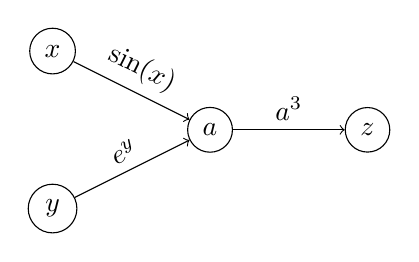
\begin{tikzpicture}

      \path (0,1) node [circle,draw](var_x){$x$};
      \path (0,-1) node [circle,draw](var_y){$y$};
      \path (2,0) node [circle,draw](var_a){$a$};
      \path (4,0) node [circle,draw](var_z){$z$};
      % \path[red] (0,1.5) node(x1){$x_1$} (0,0) node(x2){$x_2$} (0,-1.5) node(x3){$x_3$};
      \draw[->] (var_x) -- node[above,sloped]{$\sin(x)$} (var_a);
      \draw[->] (var_y) -- node[above,sloped]{$e^y$} (var_a);
      \draw[->] (var_a) -- node[above,sloped]{$a^3$} (var_z);

    \end{tikzpicture}

  \end{minipage}
  \begin{minipage}[h!]{0.5\textwidth}
    \begin{align*} % or align*
      a(x,y) &= \sin(x) + e^y \\
      z(a(x,y)) &= a^3(x,y) = \left(\sin(x) + e^y\right)^3 \\[3ex]
      \partderiv{z}{x} &= \partderiv{a}{x} \cdot  \partderiv{z}{a} = \cos(x) \cdot 3a^2 \\[0.5ex]
      \partderiv{z}{y} &= \partderiv{a}{y} \cdot \partderiv{z}{a} = e^y \cdot 3a^2
    \end{align*}
  \end{minipage}

  \caption{Computation Graph einer exemplarischen Verkettung von Funktionen}
  \label{fig:computation_graph}
\end{figure}

Der erste Schritt der Rueckwaertsprogagierung besteht darin, dass man die partiellen Ableitungen $\ipartderiv{C}{z_j^l}$
der Kostenfunktion $C$ bezueglich den gewichteten Summen $z_j^l$ aller Schichten
berechnet. Daraus laesst sich dann spaeter sehr einfach die partiellen Ableitungen
bezueglich den Gewichten $\ipartderiv{C}{w_{j,k}^l}$ und bezueglich den Neigung
$\ipartderiv{C}{b_j^l}$ berechnen.
\para{}
Zur Uebersichtlichkeit definiert man einen \keyword{Fehler} $\delta_j^L$ fuer
jeder $j$-te Neuron in jeder $l$-ten Schicht, welcher die partielle Ableitung bezueglich der
gewichteten Summe ist. Ebenfalls definiert man analog einen Fehlervektor
$\vec{\delta}^l$, welcher alle Fehler $\delta_j^l$ einer Schicht $l$
zusammenfasst. Nun heisst es diesen fuer jedes Neuron jeder Schicht zu
berechnen.

\begin{gather}
  \tag{BP0} \delta_j^l \coloneqq \partderiv{C}{z_j^l} \\
  \tag{BP0a} \vec{\delta}^l \coloneqq \trans{\begin{pmatrix} \ds\partderiv{C}{z_1^l} & \ds\partderiv{C}{z_2^l} & \cdots & \ds\partderiv{C}{z_{|l|}^l} \end{pmatrix}}
\end{gather}

Da die Kostenfunktion unmittelbar auf die letzte Schicht angewandt wird, beginnt
man auch mit der Berechnung des Fehlers in der letzten Schicht $L$.
Wir stellen nun einen Computation Graph auf, um die partiellen Ableitungen zu bilden.
\para{}

\begin{figure}[h!]
  \centering
  \begin{tikzpicture}
    \path (0,2) node [circle,draw](z1){$z_1^L$};
    \path (0,0) node [circle,draw](z2){$z_2^L$};
    \path (0,-2) node [circle,draw](z3){$z_3^L$};
    \path (3,2) node [circle,draw](a1){$a_1^L$};
    \path (3,0) node [circle,draw](a2){$a_2^L$};
    \path (3,-2) node [circle,draw](a3){$a_3^L$};
    \path (6,0) node [circle,draw](C){$C$};

    \draw[->] (z1) -- node[above,sloped]{$\varphi(z_1^L)$} (a1);
    \draw[->] (z2) -- node[above,sloped]{$\varphi(z_2^L)$} (a2);
    \draw[->] (z3) -- node[above,sloped]{$\varphi(z_3^L)$} (a3);

    \draw[->] (a1) -- node[above,sloped]{$c(a_1^L,\hat{y}_1$)} (C);
    \draw[->] (a2) -- node[below,sloped]{$c(a_2^L,\hat{y}_2$)} (C);
    \draw[->] (a3) -- node[below,sloped]{$c(a_3^L,\hat{y}_3$)} (C);

    % endings
    \node (beg1) at (-3,2) {};
    \node (beg2) at (-3,0) {};
    \node (beg3) at (-3,-2) {};

    \draw[dashed] ($(beg1)!0.6!(z1)$) -- (z1);
    \draw[dashed] ($(beg1)!0.6!(z2)$) -- (z2);
    \draw[dashed] ($(beg1)!0.6!(z3)$) -- (z3);
    \draw[dashed] ($(beg2)!0.6!(z1)$) -- (z1);
    \draw[dashed] ($(beg2)!0.6!(z2)$) -- (z2);
    \draw[dashed] ($(beg2)!0.6!(z3)$) -- (z3);
    \draw[dashed] ($(beg3)!0.6!(z1)$) -- (z1);
    \draw[dashed] ($(beg3)!0.6!(z2)$) -- (z2);
    \draw[dashed] ($(beg3)!0.6!(z3)$) -- (z3);
  \end{tikzpicture}
  \caption{Computation Graph zur Berechnung von $\delta_j^L$}
  \label{fig:cg_L}
\end{figure}
Wir koennen dem Computation Graph aus Abbildung (\ref{fig:cg_L}) entnehmen, dass die Kosten $C$ eine Funktion
in Abhaengigkeit von den letzten Aktivierungen $a_j^L$ ist, welche wiederum in
Abhaengigkeit von den gewichteten Summen $z_j^L$ berechnet werden.
Somit koennen wir mithilfe der Kettenregel folgende Beziehung aufstellen:
\begin{equation*}
  \delta_j^L = \partderiv{C}{z_j^L} = \partderiv{a_j^L}{z_j^L} \cdot \partderiv{C}{a_j^L}
\end{equation*}

Da $a_j^L$ durch die Anwendung der Aktivierungsfunktion $\varphi$ auf $z_j^L$
gebildet wrid, ist $\ipartderiv{a_j^L}{z_j^L}$ einfach die Ableitung der Aktivierungsfunktion
$\varphi'(z_j^L)$. Somit koennen wir schreiben:

\begin{equation}\tag{BP1}
  \delta_j^L = \partderiv{C}{a_j^L} \cdot \varphi'(z_j^L)
\end{equation}

Nun moechten wir diese Ausdruecke wieder in Matrixschreibweise realisieren,
welche die ganze Schicht $L$ zusammenfasst. Dazu
muss eine neue Operation eingefuehrt werden: das Hadamard-Produkt.

\begin{defbox}{Hadamard-Produkt}
  Das Hadamard-Produkt ist ein spezielles Produkt zweier gleichgrossen Matrizen
  $\mat{A} \in \set{R}^{m \times n}$ und $\mat{B} \in \set{R}^{m \times n}$.
  Die resultierende Matrix ergibt sich aus der elementweisen Multiplikation der Ausgangsmatrizen.

  \begin{minipage}{0.5\textwidth}
    \begin{equation*}
      \mat{A} \odot \mat{B} =
      \begin{pmatrix}
        \matelem{A}_{1,1} \matelem{B}_{1,1} & \cdots & \matelem{A}_{1,n} \matelem{B}_{1,n} \\[0.3em]
        \vdots & \ddots & \vdots \\[0.3em]
        \matelem{A}_{m,1} \matelem{B}_{m,1} & \cdots & \matelem{A}_{m,n} \matelem{B}_{m,n} \\[0.3em]
      \end{pmatrix}
      \in \set{R}^{m \times n}
    \end{equation*}
  \end{minipage}
  %
  \begin{minipage}{0.5\textwidth}
    \begin{equation*}
      \vec{v} \odot \vec{w} =
      \begin{pmatrix}
        v_1 w_1 \\
        \vdots \\
        v_n w_n
      \end{pmatrix}
    \end{equation*}

  \end{minipage}
\end{defbox}
\para{}

Mit $\vecf{\varphi}'$ als die vektorisierte Ableitung der Aktivierungsfunktion,
koenne wir den Fehlervektor der letzten Schicht so berechnen:

\begin{equation*}
  \vec{\delta}^L = \trans{\begin{pmatrix} \ds\partderiv{C}{a_1^L} & \ds\partderiv{C}{a_2^L} & \cdots & \ds\partderiv{C}{a_{|L|}^L}\end{pmatrix}} \odot \vecf{\varphi}'(\vec{z}^L)
\end{equation*}

Dabei ist der erste Operand des Hadamard-Produkt, nichts anderes als
der Gradient $\vecf{\nabla}_{\vec{a}^L} C$ der Kostenfunktion $C$ bezueglich dem Aktivierungsvektor
$\vec{a}^L$ der letzten Schicht. Dieser Gradient kann einfach berechnet werden, indem man die
Ableitungsfunktion fuer die gewaehlte Kostenfunktion bildet. Wuerde man die
Mittlere quadratischen Abweichung $C = \frac{1}{2}(\vec{\hat{y}} - \vec{a}^L)^2$ als Kostenfunktion waehlen, haetten wir
$\vecf{\nabla}_{\vec{a}^L} C = (\vec{a}^L - \vec{\hat{y}})$  \\
Daraus folgt folgende kompakte Gleichung fuer den Fehler der ganzen letzten Schicht:

\begin{equation}\tag{BP1a}
  \vec{\delta}^L = \vecf{\nabla}_{\vec{a}^L}C \odot \vecf{\varphi}'(\vec{z}^L)
\end{equation}

\para{}
Nun muessen wir eine rekursive Berechnungsmethode des Fehlers $\delta_j^{l-1}$
der vorherigen Schicht anhand des Fehlers $\delta_j^l$ der jetztigen Schicht
erarbeiten. Dafuer stellen wir zuallererst wieder einen Computation Graph auf.

\begin{figure}[h!]
  \centering
  \begin{tikzpicture}
    \path (0,1) node [circle,draw](z1-){$z_1^{l-1}$};
    \path (0,-1) node [circle,draw](z2-){$z_2^{l-1}$};
    \path (3,1) node [circle,draw](a1-){$a_1^{l-1}$};
    \path (3,-1) node [circle,draw](a2-){$a_2^{l-1}$};
    \path (7,2) node [circle,draw](z1){$z_1^l$};
    \path (7,0) node [circle,draw](z2){$z_2^l$};
    \path (7,-2) node [circle,draw](z3){$z_3^l$};

    \draw[->] (z1-) -- node[above,sloped]{$\varphi(z_1^L)$} (a1-);
    \draw[->] (z2-) -- node[above,sloped]{$\varphi(z_2^L)$} (a2-);

    \draw[->] (a1-) -- node[sloped,above]{$\times w_{1,1}$} (z1);
    \draw[->] (a1-) -- node[sloped,above right]{$\times w_{2,1}$} (z2);
    \draw[->] (a1-) -- node[sloped,below right]{$\times w_{3,1}$} (z3);
    \draw[->] (a2-) -- node[sloped,above right]{$\times w_{1,2}$} (z1);
    \draw[->] (a2-) -- node[sloped,above right]{$\times w_{2,2}$} (z2);
    \draw[->] (a2-) -- node[sloped,below]{$\times w_{3,2}$} (z3);

    % endings
    \node (beg1) at (-3,1) {};
    \node (beg2) at (-3,-1) {};
    \draw[dashed] ($(beg1)!0.6!(z1-)$) -- (z1-);
    \draw[dashed] ($(beg1)!0.6!(z2-)$) -- (z2-);
    \draw[dashed] ($(beg2)!0.6!(z1-)$) -- (z1-);
    \draw[dashed] ($(beg2)!0.6!(z2-)$) -- (z2-);

    \draw[dashed] (z1) -- ++(1.5,0);
    \draw[dashed] (z2) -- ++(1.5,0);
    \draw[dashed] (z3) -- ++(1.5,0);

  \end{tikzpicture}
  \caption{Computation Graph zur Berechnung von $\delta_j^{l-1}$}
  \label{fig:cg_L}
\end{figure}

Es gilt erneut folgende Gleichung fuer die Berechnung des Fehlers $\delta_j^{l-1}$:
\begin{equation*}
  \delta_j^{l-1} = \partderiv{C}{z_j^{l-1}} = \partderiv{a_j^{l-1}}{z_j^{l-1}} \cdot \partderiv{C}{a_j^{l-1}}
\end{equation*}

Beim Uebergang der Schicht ($l-1$) zur Schicht $l$ beinflusst jene Aktivierungen
$a_j^{l-1}$ alle gewichtete Summen $z_k^l$, daher folgt mit der Kettenregel,
dass die partielle Ableitung $\ipartderiv{C}{a_j^{l-1}}$ die Summe aller
$\ipartderiv{z_k^L}{a_j^{l-1}} \cdot \ipartderiv{C}{z_k^l}$ sein muss.

Somit erhalten wir:
\begin{equation*}
  \delta_j^{l-1} = \varphi'(z_j^{l-1}) \cdot \sum_{n=1}^{|l|} \left( \partderiv{C}{z_n^l} \cdot \partderiv{z_n^l}{a_j^{l-1}} \right)
\end{equation*}

Da bei der Bildung der gewichteten Summe $z_j^l$ wird die Aktivierung
$a_k^{l-1}$ einfach mit der Gewicht $w_{n,j}^{l-1}$ multipliziert. Somit ist das
Gewicht gerade die partielle Ableitung. Ausserdem ist der Term
$\ipartderiv{C}{z_j^l}$ per Definition der Fehler $\delta_j^l$.

\begin{equation}\tag{BP2}
  \delta_j^{l-1} = \varphi'(z_j^{l-1}) \cdot \sum_{n=1}^{|l|} \left( w_{n,j}^{l-1} \cdot \delta_m^l \right)
\end{equation}

Auch diese Gleichung haetten wir gerne in der Matrixschreibweise. Wir beginnen
mit der Erweiterung auf alle gewichteten Summen.

\begin{equation*}
  \vec{\delta}^{l-1} = \vecf{\varphi}'(\vec{z}^{l-1}) \odot \trans{\begin{pmatrix} \ds\sum_{n=1}^{|l|} w_{1,n}^{l-1} \cdot \delta_n^l & \cdots & \ds\sum_{n=1}^{|l|} w_{|l-1|,n} \cdot \delta_n^l \end{pmatrix}}
\end{equation*}

Der zweite Operant des Hadamard-Produkts ist hierbei gerade das Produkt der
Matrixmultiplikation zwischen
der transponierten Gewichtsmatrix $\trans{(\mat{W}^{l-1})}$ der Schicht ($l-1$)
und dem Fehlers $\vec{\delta}^l$ der Schicht $l$.

GEWICHTSMATRIX INDIZES STIMMEN WAHRSCHEINLICH NICHT
\begin{gather*}
  \trans{\begin{pmatrix} \ds\sum_{n=1}^{|l|} w_{1,n}^{l-1} \cdot \delta_n^l & \cdots & \ds\sum_{n=1}^{|l|} w_{|l-1|,n} \cdot \delta_n^l \end{pmatrix}} =
  \begin{pmatrix}
    w_{1,1}^{l-1} & w_{2,1}^{l-1} & \cdots & w_{|l-1|,1}^{l-1} \\
    w_{1,2}^{l-1} & w_{2,2}^{l-1} & \cdots & w_{|l-1|,2}^{l-1} \\
    \vdots & \vdots & \ddots & \vdots \\
    w_{1,|l|}^{l-1} & w_{2,|l|}^{l-1} & \cdots & w_{|l-1|,|l|}^{l-1}
  \end{pmatrix}
  \trans{\begin{pmatrix} \delta_1^l & \cdots & \delta_{|l|}^l \end{pmatrix}} \\=
  \begin{pmatrix}
    w_{1,1}^{l-1} & w_{1,2}^{l-1} & \cdots & w_{1,|l|}^{l-1} \\
    w_{2,1}^{l-1} & w_{2,2}^{l-1} & \cdots & w_{2,|l|}^{l-1} \\
    \vdots & \vdots & \ddots & \vdots \\
    w_{|l-1|,1}^{l-1} & w_{|l-1|,2}^{l-1} & \cdots & w_{|l-1|,|l|}^{l-1}
  \end{pmatrix}
  \vec{\delta}^l = \trans{(\mat{W}^{l-1})} \vec{\delta}^l
\end{gather*}

Alles in Allem erhalten wir:
\begin{equation}\tag{BP2a}
  \vec{\delta}^{l-1} = (\trans{(\mat{W}^{l-1})} \vec{\delta}^l) \odot \vecf{\varphi}'(\vec{z}^{l-1})
\end{equation}

\para{}

Nun gilt es noch die partiellen Ableitungen fuer die Gewichte und die Neigungen
durch den Fehler $\delta_j^l$ auszudruecken.
Zuerst einmal fuer die Neigung gilt:
\begin{equation*}
  \partderiv{C}{b_j^l} = \partderiv{C}{z_j^{l+1}} \partderiv{z_j^{l+1}}{b_k^l}
\end{equation*}
Der erste Term ist hierbei per Definition unser Fehler $\delta_j^l$ und der
zweite Term laesst sich zu 1 evaluieren, da die Summe $z_k^{l+1}$ nur aus
$b_k^l$ und sonstigen Konstanten Termen besteht.
Somit ist die Ableitung der Neigung gerade unser Fehler:
\begin{equation}\tag{BP3}
  \partderiv{C}{b_j^l} = \delta_j^l
\end{equation}
Somit ist der Kostengradient bezuglich der Neigung gerade der Fehlervektor.
\begin{equation}\tag{BP3a}
  \vecf{\nabla}_{\vec{b^l}} C =  \vec{\delta}^l
\end{equation}

Fuer die partiellen Ableitungen der Kosten nach dem Gewicht giltet:
\begin{equation}\tag{BP4}
  \partderiv{C}{w_{j,k}^l} = \partderiv{C}{z_k^{l+1}} \partderiv{z_k^{l+1}}{w_{j,k}^l} = \delta_k^{l+1} \cdot a_j^l
\end{equation}

Uns somit ist der Graidient der Kosten respektive einer Gewichtmatrix:
UEBERPRUEFEN
\begin{equation}\tag{BP4a}
  \vecf{\nabla}_{\mat{W}^l} C = \vec{\delta}^{l+1} \trans{(\vec{a^l})}
\end{equation}


\cite{Nielsen}


\section{Universal Approximation Theorem}\label{sec:UAT}
Neural Network kann alles erlernen

\section{Vanishing Gradient Problem}

Gleichung BP1 sagt uns, dass der Lernprozess langsam ist, falls $\varphi$ fast 0
oder 1 ist. Sigmoid. Das Neuron ist saturiert und lernt nicht mehr. In letzter Schicht

\subsection{Kreuzentropie-Kostenfunktion}

\subsection{ReLU}

\pagebreak
\chapter{Convolutional Neural Networks}
Viele Anwendungen von Machine Learning sind verbunden mit Bild- oder
Audioverarbeitung, wie z.B Bildklassifizierung, Gesichtserkennung oder
Spracherkennung.
Vorallem aber fuer hochaufloesende Bilder sind die KNNs, die wir soeben
kennengelernt haben, nicht geeignet. Sie sind zum Teil gar nicht in der
Lage eine Korrelation zwischen den Inputs und Outputs zu erlernen.
Um diesen Umstand zu erklaeren, wird nun ein kleines Beispielmodell erlauetert:
\para{}
Es soll ein KNN designed werden, welches eine Photographie klassifizieren
soll, ob darauf ein Hund sichtbar ist oder nicht. Wir nehmen fuer dieses
Gedankenexperiment bereits ein relativ niedrig aufgeloestes Bild mit $256 \times 256$
Pixel, dies entspricht weniger als $0.07$ Megapixel (ein iPhone XS hat eine Kamera mit
12 Megapixel). Um die verschiedenen Farben zu codieren besitzt jeder Pixel drei Komponten R, G
und B. Somit hat dieses Bild insgesamt $256 \times 256 \times 3 = 196'608$
Komponenten. Jede Komponente ist ein Feature welches das KNN zu verrechnen hat. Somit bestuende
die erste Schicht des Netzwerkes aus fast $200'000$ Neuronen. Um diese Schicht
nun mit seiner Nachbarsschicht, welche gleiche Dimensionen besitzt, zu verbinden, braucht
es $196'608 \times 196'608 = 38'654'705'664$ Verbindungen und damit gleich so
viele Gewichte! Fuer ein Netwerke ohne eine einzige Zwischenschichten gaebe es
also ueber 38 Milliarden Modellparameter zu erlernen! Das dies nicht realistisch ist,
sollte auf der Hand liegen.
\para{}
Nicht nur die Anzahl Modellparameter sind ein Problem fuer KNNs in der
Bildverarbeitung, sondern es bestehen noch weiter Probleme.
Trotzdem sollte nun klar sein, dass eine andere Modellarchitektur noetig ist, um Machine
Learning auf Bilder anzuwenden. Fuer genau solche Anwendungen wurde eine modifizierte
Version eines KNNs entwickelt: das \keyword{Convolutional Neural Network} (CNN).
Im Allgemeinen sind CNNs immer geeignet, um Daten zu verarbeiten, welche eine
rasterartige Form haben, wie eben z.B Bilder.
Diese Art von Netzwerk, macht Gebrauch von Konzepten aus der klassischen
Bildverarbeitung, wie sie mit beispielsweise Photoshop gemacht werden kann.
Wie beim Perzeptron und bei den klassischen KNNs auch, ist die Architektur
biologisch inspiriert.
Der folgende Abschnitt wird die Funktionsweise eines solchen CNNs erklaeren.
\para{}
\cite{Goodfellow-et-al-2016}
\cite{deeplearning.ai:cnn}
\cite{wiki:cnn}

\section{Bilder als Tensoren}
CNNs operieren an Bildern. Sie stellen den Input fuer die Modells dar.
Um mit ihnen rechnen zu koennen, ist es sinnvoll sie als sogennante
\keyword{Tensoren} vom Rang 3 zu untersuchen, anstatt sie als Anordnungen von
Pixeln zu betrachten. \\
Um zu verstehen, was ein Tensor dritten Ranges ist, muessen wir zuerst verstehen, was ein Tensor im Allgemeinen ist.

\begin{defbox}{Tensor}
  Ein Tensor $\ten{T}$ ist eine Verallgemeinerung von Skalaren, Vektoren und Matrizen auf
  $n$ Dimensionen. Es handelt sich wie bei Matrizen um
  eine Zahlenanordnung. Dabei wird die Anzahl Dimensionen, innerhalb welchen die
  Zahlen liegen als Rang oder Stufe $n$ des Tensors bezeichnet. Vorstellen kann man sich einen Tensor
  als ein Hyperrechteck mit $n$ Dimensionen, innerhalb dessen die Zahlen in
  einem Raster angeordnet sind. Diese Zahlen sind die Elemente des Tensors.
  Ein Tensor nullten Ranges ist ein Skalar, einer erster Stufe ein Vektor und
  einer mit Rang 2 ist eine normale Matrix.
  \begin{gather*}
    1 \in \set{R} \text{ (Skalar)} \quad \begin{pmatrix} 1 & 2 & 3 \end{pmatrix}
    \in \set{R}^3 \text{ (Vektor)} \quad
    \begin{pmatrix}
      1 & 2 & 3 \\
      4 & 5 & 6 \\
    \end{pmatrix} \in \set{R}^{2 \times 3} \text{ (Matrix)}
  \end{gather*}


\end{defbox}

\begin{defbox}{Tensor 3. Ranges}
  Eine Tensor $\ten{T} \in \set{R}^{h \times w \times d}$ mit Rang 3 ist eine 3-dimensionale Zahlenanordnung. Man kann sich
  diesen Tensor einfach als eine 3D-Matrix vorstellen. Ein Volumen innerhalb
  dessen Zahlen in einem Raster angeordet sind.
  Analog zum Volumen, bezeichnet man die Form des Tensors mit Hoehe, Breite und
  Tiefe. \\
  Ein Tensor von der Form $\set{R}^{3 \times 3 \times 3}$ koennte folgendermassen
  aussehen:
  \para{}

  % \newcommand{\arrayfilling}[2]{
  % \fill[#2!30, opacity=.5] ([shift={(1mm,1mm)}]#1.north west) coordinate(#1auxnw)--([shift={(1mm,1mm)}]#1.north east)coordinate(#1auxne) to[out=-75, in=75] ([shift={(1mm,-1mm)}]#1.south east)coordinate(#1auxse)--([shift={(1mm,-1mm)}]#1.south west)coordinate(#1auxsw) to[out=105, in=-105] cycle;
  % \fill[#2!80!black, opacity=1] (#1auxne) to[out=-75, in=75] (#1auxse) to[out=78, in=-78] cycle;
  % \fill[#2!80!black, opacity=1] (#1auxnw) to[out=-105, in=105] (#1auxsw) to[out=102, in=-102] cycle;
  % }

  %   \begin{tikzpicture}[font=\ttfamily,
  %     mymatrix/.style={
  %     matrix of math nodes, inner sep=0pt, color=#1,
  %     column sep=-\pgflinewidth, row sep=-\pgflinewidth, anchor=south west,
  %     nodes={anchor=center, minimum width=5mm,
  %     minimum height=3mm, outer sep=0pt, inner sep=0pt,
  %     text width=5mm, align=right,
  %     draw=none, font=\small},
  %   }
  %     ]

  %     \matrix (C) [mymatrix=green] at (6mm,5mm)
  %     {0 & 1 & 0 \\ -1 & 0 & 0\\ 0 & 0 & 0\\};
  %     \arrayfilling{C}{green}

  %     \matrix (B) [mymatrix=red] at (3mm,2.5mm)
  %     {0 & 0 & -1 \\ 0 & 0 & 0\\ 1 & 0 & 0\\};
  %     \arrayfilling{B}{red}

  %     \matrix (A) [mymatrix=blue] at (0,0)
  %     {0 & 0 & 0 \\ 0 & 0 & 1\\ 0 & -1 & 0\\};
  %     \arrayfilling{A}{blue}

  %     \foreach \i in {auxnw, auxne, auxse, auxsw}
  %     \draw[brown, ultra thin] (A\i)--(C\i);

  %     \node[left=1mm of B.west] {$\ten{T} =$};
  %     \node[right=3mm of B.east] {$\in \set{R}^{3 \times 3 \times 3}$};
  %   \end{tikzpicture}

\end{defbox}

\para{}
Ein Bild kann somit einfach als Tensor dritten Ranges $\ten{B} \in \set{R}^{h
  \times w \times c}$, der Form $(\text{Bildhoehe} \times \text{Bildbreite}
\times \text{Anzahl Farbkomponenten})$ betrachtet werden.
Elemente der Matrix nehmen dann einfach die Werte der Pixelkomponenten an.
Ein schwarzweiss Bild hat nur eine Komponente, welche die Helligkeit angibt.
Somit waere es eine normale 2D-Matrix $\mat{B} \in \set{R}^{h \times w}$.
Siehe Abb. (\ref{fig:bildmatrix}).
\para{}


\begin{figure}[h!]
  \begin{tikzpicture}

  \end{tikzpicture}
  \caption{Beispiel einer Bildmatrix}
  \label{fig:bildmatrix}
\end{figure}

\section{Topologie von CNNs}
Ein CNN besteht, wie ein KNN auch, aus Schichten. Jede dieser Schichten erhaelt
ein Bild als Input und hat auch wieder eines als Output. Somit nehmen die Bilder
die Rolle der Aktivierungen $a$ ein, weshalb man sie mit $\ten{A}^l$ bezeichnet.
Das Bild $\ten{A}^0$ ist hierbei wieder der Input $\ten{X}$ ins ganze Netz.
\para{}
Ein wichtiger Unterschied eines CNNs ist, dass es verschiedene Typen von
Schichten gibt. Man unterscheiden zwischen drei Arten von Schichten:
\begin{itemize}
\item{\keyword{Fully-connected Schichten},}
\item{\keyword{Convolutional Schichten}, und}
\item{\keyword{Pooling Schichten}.}
\end{itemize}
Die fully-connected Schicht ist altbekannt und ist einfach die klassischen Schicht
eines KNNs, bestehend aus Neuronen.
Die Convolutional Schicht und die Pooling Schicht sind zwei neuartige Schichten,
welche eine Erweiterung fuer CNNs darstellen. Sie werden in diesem Kapitel erklaert.
Diese beide neuen Arten von Schichten bildet gewissermassen eine Einheit, denn
auf eine Convolutional Schicht folgt auch immer eine Pooling Schicht.

\para{}
In Abbildung (\ref{fig:cnn_topology}) ist ein Schema eines CNNs abbgebildet.
\begin{figure}[h!]

  \caption{Schichtung eines CNNs}
  \label{fig:cnn_topology}
\end{figure}



\section{Filter}
Zuerst betrachten wir die Convolutional Schicht. Diese Schicht macht ausgiebig
Gebrauch von sogennanten Filtern. Diese werden in diesem Abschnitt behandelt.

\subsection{Filter in der Bildverarbeitung}
\keyword{Filter} (auch Kerne) sind in der Bildverarbeitung sehr verbreitet. Jeder kennt sie entweder
von Photoshop, von Instagram oder sonstigen Bildbearbeitungsprogrammen.
Auch CNNs machen Gebrauch von solchen Filtern, in diesem Fall um die Features eines Bildes zu
erlernen. Aus diktaktischen Gruenden betrachten wir zuerst nur 2D-Filter, welche sich fuer graustufige
Bilder $\mat{B} \in \set{R}^{h \times w}$ eignen.
\begin{figure}[h!]

  \caption{der Instagramfilter: Blablabla}
\end{figure}

\para{}
Ein Filter ist einfach eine Regionen, deutlich kleiner als das verarbeitete Bild, welche
ueber alle Pixel wandert, diese manipuliert und so wieder ein neues Bild
$\mat{B}^*$ liefert.
Mathematisch gesehen handelt es sich bei einem Filter einfach um einen Tensor,
den sogennanten \keyword{Filtertensor} oder Faltungstensor (siehe Abb.
(\ref{fig:filtermatrix})). Fuer unser graustufiges Bild ist dieser eine 2D-Matrix,
bezeichnet mit $\mat{F} \in \set{R}^{f \times f}$. Solche Filter sind immer quadratisch,
wobei ihre Zeilen- bzw. Spaltenlaenge mit $f$ bezeichnet wird. Dabei ist $f$
immer eine ungerade Zahl, damit ein Element, das sogennante \keyword{Zentralelement}, immer im Zentrum des Filters liegt.

\begin{figure}[h!]
  % Zentralelement kennzeichnen
  \caption{eine 2D-Filtermatrix}
  \label{fig:filtermatrix}
\end{figure}
\para{}
Das Verhalten des Filters wird durch seine Matrixeintraege bestimmt.
Die Elemente koennen also so gewaehlt werden, dass wenn der Filter auf ein Bild
angewandt wird, er bestimmte Features aus dem Bild hervorhebt. Solche Features
koennten zum Beispiel Raender oder Kanten sein, welche betont werden.
\para{}
Ein gutes Beispiel ist der Sobel-Filter. Er ist ein typischer Kantendetektions-Filter mit einer
Groesse von $f = 3$. Wir betrachten nun den Sobelfilter $\mat{G}_x$, welcher
horizontale Kanten akzentuiert. Die Eintraege dieses Filters lauten wie folgt:
\begin{equation*}
  \mat{G}_x =
  \begin{bmatrix}
    -1 & 0 & +1 \\
    -2 & 0 & +2 \\
    -1 & 0 & +1 \\
  \end{bmatrix}
\end{equation*}

Angewandt auf ein Bild, erhaelt man ein neues Bild, bei welchem alle erkannten
Katen weiss eingefaerbt sind und die restlichen Bereichen schwarz sind.
Der Filter erkennt dabei jede Stelle als Kante, welche zwei Regionen mit
genug grossem Kontrast voneinander trennt.
In Abbildung (\ref{fig:sobel_filter}) wurde der horizontale Sobelfilter auf ein
Beispielbild angewandt. Links ist das Ursprungsbild und rechts ist das
prozessierte Bild.


\begin{figure}[h!]

  \caption{Sobel-Filter angewandt auf Beispielsbild}
  \label{fig:sobel_filter}
\end{figure}

\para{}
\cite{wiki:sobel_operator}
\cite{deeplearning.ai:cnn}
\cite{wiki:kernel}


\subsection{Filter in CNNs}
Wie wir vorhin erfahren haben, koennen Filter genutzt werden um gewisse
Features eines Bildes hervorzuheben und andere Features zu ignorieren. Dabei
bestimmen die Filtereintraege, welche Features extrahiert werden. Somit bestimmt
die Aufgabe darin, die richtigen Filterelemente zu bestimmen, damit die
gewuenschten Features erkannt werden und auf die gewuenschten Outputs abgebildet
werden. Daraus schliesst sich, dass die Filtereintraege die Modellparameter
eines CNNs sind. Mithilfe des Gradietenverfahrens soll erneut diese Parameter
erlernt werden. \\
Da die Filter die gleiche Funktion haben, wie die Gewichte in einem KNN,
bezeichnet man die Filter in einem CNN mit $\ten{W}$.

\begin{equation*}
  \mat{W} = \begin{pmatrix}
    w_{1,1} & \cdots & w_{1,f} \\
    \vdots & \ddots & \vdots \\
    w_{f,1} & \cdots & w_{f,f}
  \end{pmatrix}
\end{equation*}

Die Groesse der Filters bzw. die Groesse der rezeptiven Felder ist
ein Hyperparameter.
\para{}


\subsection{Filteroperation intutitiv}\label{sec:filteroperation_intutitiv}
Wie wendet man nun einen solchen Filter auf ein Bild an? Um das Prozedere einer
Filteroperation leichter verstaendlich zu machen, wird sie erneut fuer ein
graustufiges Bild $\mat{A} \in \set{R}^{h \times w}$ erlauetert. Spaeter werden auch noch farbige
Bilder erklaert.
\para{}
Bei einer Filteroperation, wendet man einen Filter $\mat{W}$ auf eine Bildmatrix
$\mat{A}$ an und erhaelt so ein neues Bild $\mat{A}^*$. Man schreibt dafuer:
$\mat{A}^* = \mat{W} * \mat{A}$. \\
Um nun diese Operation zu erklaeren, verwenden wir als Beispiel eine
2D-Filtermatrix $\mat{W} \in \set{R}^{3 \times 3}$, bei welcher
$f = 3$ gewaehlt wurde.
Wie bereits vorhin erwaehnt wandert der Filter ueber das Bild. Dabei befindet
sich der Filter immer ueber einer Region des Bilder, welche gleich gross ist,
wie der Filter selber (in diesem Fall ($3 \times 3$)), so dass den Filtermatrixeintraegen immer eindeutig
Bildmatrixeintraege entsprechen. Diese Region des Bildes bezeichnet man als das
\keyword{Rezeptive Feld} des Filters (siehe Abb. (\ref{fig:receptive_field})). Wir schreiben dafuer
$\tilde{\mat{A}}^{(y,x)}$, wobei die hochgestellten Indizes $(y,x)$ die Position
des Zentralelements im rezeptiven Feldes angiebt. Somit ist das rezeptiven Feld einfach eine
Untermatrix $\tilde{\mat{A}} \in \set{R}^{3 \times 3}$ des Obermatrix $\mat{A}$.

\begin{figure}[h!]

  % Zentralelement einzeichnen mit Beschriftung
  \caption{ein Filter und sein rezeptives Feld}
  \label{fig:receptive_field}
\end{figure}

\para{}
Der Filter beginnt nun oben links ueber das Bild zu wandern. Somit
hat der Filter zu beginn das rezeptive Feld $\tilde{\mat{A}}^{(2,2)}$, denn der
Filter darf nicht ueber die Raender des Bildes hinausragen.
Nun werden die Elemente der Filters mit den Elementen des rezeptiven Feldes
verrechnet, welche die gleichen Dimensionen besitzen. Dabei wird einfach das
Hadamard-Produkt (das elementweise Produkt) des beiden Matrizen miteinander
gebildet. Nun erhalten wir eine neue Matrix $\mat{W} \odot
\tilde{\mat{A}}^{(2,2)} = \mat{P} \in \set{R}^{3 \times 3}$.
Nun werden noch alle Elemente der neuen Matrix $\mat{P}$
aufsummiert. Diese Zahl ist dann der Grauwert des ersten Pixels $(\mat{A}^*)_{1,1}$ des bearbeiteten
Bildes. In diesem Sinne stellt der Filter eine Gewichtung der Nachbarspixel dar, welche
bestimmt, wie die neuen Pixel aussehen.
\begin{equation*}
  (\mat{A}^*)_{1,1} = \sum_{y=1}^3 \sum_{x=1}^3 (\mat{P})_{y,x}
\end{equation*}

Nun wird der Filter um ein Element nach rechts verschoben und die gleiche
Prozedur angewendet, um den zweiten Pixel zu berechnen. Dies
wird durchgezogen, bis eine ganze Zeile der Bildmatrix durchstreift wurde.
Danach wird der Filter wieder nach ganz rechts verschoben und er bewegt sich ein
Element nach unten. Das geschieht, bis das ganze Bild verrechnet wurde.
Dabei werden die Elemente des urspruenglichen Bildes durchaus mehrmals
verrechnet, da es zu einer Ueberlappung des vorherigen Filter und des
verschobenen Filters kommt.

\begin{figure}[h!]

  \caption{Schema, wie ein Filter ueber ein Bild laueft}
\end{figure}

Es ist zu bemerken, dass das neue Bild $\mat{A}^* \in \set{R}^{(h-2) \times (w-2)}$ nicht mehr die gleichen Masse
hat, wie das Ursprungsbild $\mat{A} \in \set{R}^{h \times w}$. Das liegt daran, dass pro
Lage des Filters jeweils ein Pixel des neuen Bildes berechnet wird. Man kann
sich vorstellen, dass an der Position des Zentralelements jeweils ein neuer
Pixel entsteht. Dabei muss der Filter immer eine vollstaendige Region als
rezeptives Feld haben. Dadurch kommt das Zentralelement nie auf den Raendern des
Bilds zu liegen. Somit fallen diese weg.
\para{}
\cite{deeplearning.ai:cnn}
\cite{wiki:convolution}

\subsection{Filteroperationen als diskrete Faltungen}
Eigentlich handelt es sich bei einer Anwendung eines Filters auf ein Bild um
eine spezifische mathematische Operation: eine \keyword{diskrete Faltung} (engl.:
\keyword{Convolution}).
\footnote{
  Eigentlich ist die Filteroperation keine richtige Faltung im mathematischen
  Sinne, sondern eher eine sogennante Kreuzkorrelation. Dennoch wird im Verlauf
  dieser Arbeit der Begriff Faltung im Zusammenhang mit Filteroperationen verwendet.\\
  Fuer Intressierte: Die Kreuzkorrelation funktioniert gleich wie eine Faltung,
  jedoch wird die eine Matrix zuerst horizontal, wie auch vertikal gespiegelt,
  bevor die eigentliche Faltung angewandt wird.
}
Daher ruehrt auch der Name des Convolutional Neural Networks.
Wir werden die Faltung als mathematische Operation nicht im vollen Umfang
betrachten, da sie relativ kompliziert ist. Wir werden uns lediglich auf die
Bedeutung der Faltung fuer Filter beschraenken.
Damit ihr die Defintion trotzdem mal gesehen habt:
\begin{equation}
  (f * g)(x) = \int f(t) g(x-t) \text{d}a = \sum_{t=-\infty}^\infty f(a)g(x-t)
\end{equation}
\para{}
Streng genommen wird in CNN nicht eine diskrete Faltung durchgefuehrt, sondern
eine sogennante Kreuzkorrelation. Der Unterschied dabei ist, dass bei einer
Kreuzkorrelation die Faltungsmatrix nicht zuerst horizontal, wie auch vertiakl
gespiegelt wird. Begrifflich benutzt man jedoch Faltung/Convolution um beide
Operationen zu bezeichnen.

\para{}

Mithilfe der Faltungoperation koennen wir die Schritte welche in Sektion
(\ref{sec:filteroperation_intuitiv}) erklaert wurden zusammenfassen. Um die
Schreibweise etwas zu vereinfachen, fuehren wir folgende Konvention ein:
\[ \mat{M}(x,y) = (\mat{M})_{y,x}\]
Um einen Pixel $\mat{A}^*(x,y)$ des neuen Bildes zu berechnen, benutzt man folgende Formel.

Kreuzkorrelation
\begin{equation}
  \mat{A}^*(x,y) = (\mat{W} * \mat{A})(x,y) = \sum_{u=0}^f \sum_{v=0}^f \mat{A}(x+u,y+v)\mat{W}(u,v)
\end{equation}


Fuer farbige Bilder ist das Vorgehen praktisch das selbe. Es werden nun
lediglich 3D-Tensoren anstatt 2D-Tensoren verwendet. Wir betrachten den
allgemeinen Bildtensor $\ten{A}_{h \times w \times c}$, wobei $c$ die Anzahl
Farbkomponenten (engl.: channels) ist.
Nun benutzt man Filter $\ten{W}_{f \times f \times c}$ mit beliebiger Groesse
$f$ aber mit der gleicher Tiefe $c$ wie das Ursprungsbild $\mat{A}$.
Das heisst der Filter muss nicht entlang der Tiefe des Bildes wandern, da er
gerade gleich tief ist, wie das Bild. \\
Die allgemine Filtergleichung lautet:
\begin{equation}
  \ten{A}^*(x,y,z) = (\ten{W} * \ten{A})(x,y,z) = \sum_{u=0}^f \sum_{v=0}^f \sum_{w=0}^c \mat{A}(x+u,y+v,w)\mat{W}(u,v,w)
\end{equation}


\subsection{Padding}
Wie bereits erwaehnt schrumpfen die Bilder (an den Raendern), wenn man ein Filter auf sie anwendet.
Zur Erinnerung: Dies liegt daran, dass pro Lage des Zentralelement nur ein Pixel
des neuen Bildes entsteht und das Zentralelement nunmal nicht auf allen
Ursprungspixeln zu liegen kommt. Die Raender fallen so weg. Diese Groesse des
Wegfalls haengt von der Filtergroesse $f$ ab. Hierbei giltet folgende Formel fuer die
neue Groesse $n_1$ des Bildes, anhand der alten Groesse $n_0$.
\begin{equation}
  n_1 = n_0 - f + 1
\end{equation}

Das Problem hierbei ist, dass nach einigen Faltungen das Bild extrem geschrumpft
ist und im Grenzfall kleiner als der Filter wird. Das darf natuerlich nicht
passieren. Ausserdem geht dabei Information an den Raender verloren, da es im
Innern des Bildes zu viel Overlapping der Filterlagen kommt und die Raeder nur
sehr wenig einbezogen werden.
\para{}
Diese Probleme werden mit sogennantem \keyword{Padding} behoben. Padding ist ein
Schritt, welcher vor der eigentlichen Faltung stattfindet. Dabei werden einfach
zusatzliche Raender (Zeilen und Spalten) an das Ursprungsbild angebracht. Die
Matrix wird an den Enden erweitert. Die neuen Elemente werden dabei auf den Wert
$0$ gesetzt.

\begin{figure}[h!]

  \caption{Padding}
\end{figure}

Das Padding $p$ ist eine Zahl, welche angibt wieviele Elemente an allen Raendern
hinzugefuegt werden. Padding $p = 1$ bedeutet, dass an allen Kanten jeweils eine
Reihe bzw. Spalte hinzugefuegt wird.
Begrifflich unterscheidet man zwei Arten von Padding:
\begin{itemize}
\item{valid-Padding: Es werden keine zuesaezlichen Elemente angebracht. $f$ ist also 0.}
\item{same-Padding: Es werden so viele Reihen und Spalten angebracht, dass
    sich die Groesse des Bildes bei der Faltung erhalten bleibt.}
\end{itemize}

Um same-padding zu erhalten, muss man $p$ so waehlen, dass es den Wegfall durch
den Filter gerade kompensiert. Da durch das Padding der Filter jeweils um zwei
$p$ groesser wird, erhalt man $n_1 = n_0 - f + 1 + 2p$. Wenn man diese Formel
jetzt nach $p$ aufloest, erhaelt man folgende Formel fuer das Waehlen des
valid-Paddings $p$.
\begin{equation}
  p = \frac{f-1}{2}
\end{equation}

\subsection{Stride}
Bis jetzt haben wir bei den Filterfaltungen, den Filter pro Anwendung immer nur
um einen Pixel verschoben. Das muss aber nicht so sein. Man kann den Filter
auch mit einer anderen Schrittgroesse verschieben. Diese Eigenschaft bezeichnet
man als \keyword{Stride} $s$. Falls $s = 2$ gewaehlt wird, bedeutet das, dass der
Filter sich pro Matrixmultiplikation um zwei Elemente bewegt. Somit wurde eine
Position uebersprungen. Zur Folge hat dies, dass das neue Bild $\mat{B}^*$
deutlich kleiner geworden ist, denn das Zentralelement uebspringt somit auch
diese Felder und bildet so deutlich weniger Pixel.
\para{}
Folgende Formel beschreibt die Dimensionen des neuen Bildes $\mat{B}^*$ unter
beruecksichtigung der Filtergroesse $f$, dem Padding $p$ und dem Stride $s$.
\begin{equation}
  n_1 = \frac{n_0 + 2p - f}{s} + 1
\end{equation}

\subsection{Mehrere Filter}
Eine Filteroperation ist nicht auf einen einzigen Filter beschraenkt. Es koennen
mehrere Filter auf das gleiche Ausgangsbild angewandt werden und zusammen ein
Endbild erzeugen.
\para{}
Die Anzahl Filter bezeichnen wir mit $c$.
Nun macht man pro Filter eine Faltung ueber das Ursprungsbild $\ten{B}$, wobei
jede Faltung eine neue Matrix $\mat{B}^*_i$ liefert, wobei $i$ der Index des
Filters ist. All diese Tensoren sind zweidimensional, unabhaengig davon, wieviel
Komponten das Ursprungsbild hatte. Aus diesem Grund koennen die einzelnen
Matrizen $\mat{B}^*_i$ aufeinander gelegt werden und somit einen grossen 3D-Endtensor
$\ten{B}^*$ bilden.
Hierfuer muessen alle Filter gleich gross sein.
Die Tiefe des neuen Bildes $\ten{B}^*$ ist jetzt gerade die Anzahl Filter $c$.
Wir haben vorhin bereits immer die Tiefe des Bildes (bzw. die Anzahl
Farbkomponenten) mit $c$ bezeichnet.

\subsection{Wieso Filter?}
Es stellt sich nun die Frage, weshalb sich Filter fuer Machine
Learning eignen.
Wie bereits erwaehnt besteht die Aufgabe von Filtern darin bestimmte Features
eines Bildes hervorzuheben und die restlichen auszublenden. Genau die gleiche
Aufgabe erfuellen die Neuronen in einem KNNs. Auch sie sollen Features der
Inputsdaten erlernen, wobei gewisse Neuronen auf gewisse Features reagieren.
\para{}
Jedoch ist zu erkennen, dass Bilddaten sich deutlich von sonstigen Daten unterscheiden.
Bildfeatures bzw. Pixel sind immer im Kontext von ihren Nachbarn wichtig. Denn
ein Pixel ist erst eine Kante oder eine Ecke, wenn er zwei verschiedene
Kontraste voneinander trennt. Oder um die Konturen eines Gegenstandes zu
erkennen, muss man eine ganze Fuelle von Pixeln betrachten. Man bezeichnet
dies als \keyword{lokalisierte Features}.
\para{}
Ein weiterer Aspekt besteht darin, dass Bildausschnitt nicht immer gleich
orientiert sind. Wenn man ein Gesicht auf einem Bild erkennen moechte, sollte es
keine Rolle spielen, wo auf dem Bild es sich befindet, oder welche Groesse es
hat. Es besteht der Wunsch nach \keyword{Invarianz}. Typische Invarianzen,
welcher ein Filter erfuellt, sind: Translationinvarianz, Rotationsinvarianz und Helligkeitsinvarianz.

\keyword{Parameter Sharing}

Variable Inputgroesse, verschieden grosse Bilder

Sparse connectivity: Nicht alle Werte werden miteinander verrrechnet deutlich
schneller als Matrixmultiplikation.

\section{Convolutional Layer}
Da wir nun die Filter in ihrem vollen Umfang betrachtet haben, koennen wir uns
endlich den Convolutional Schichten widmen.
Eine ConvSchicht $l$ erhaelt als Input ein Bild $\ten{A}^{l-1} \in \set{R}^{h^{l-1}
  \times w^{l-1} \times c^{l-1}}$. Darauf werden
als erstes alle $c^l$ Filter $F_i^l \in \set{R}^{f^l \times f^l \times c^{l-1}}$ angewandt. Die neuen Matrizen $A^*_i$
werden aufeinander draufgelegt und bilden den Tensor $\ten{A}^{*,l} \in \set{R}^{h^l
  \times w^l \times c^l}$.
Nun kommt ein Optionaler Zwischenschritt. Man kann nun auf jedes Element des
Ausgangstensor einen Bias $b$ draufaddieren. \\
Nun wendet man auf alle Elemente des Ausganstensor die vektorisierte
Aktiverungsfunktion $\varphi$ an. Die gaengiste Aktiverungsfunktion ist hierfuer
die ReLU-Aktiverungsfunktion $\varphi^{ReLU}$. Dadurch erhaelt man den
Aktiverungstensor $\ten{A}^l \in \set{R}^{h^l \times w^l \times c^l}$.




Da die Faltungsoperation eine lineare Operation, braucht man wieder eine Aktivierungsfunktion.

Eigentlich ist ein CNN einfach ein KNN, welches in einer Schicht anstatt
Matrixmultiplikation eine Faltungsooperation benutzt.

\cite{Goodfellow-et-al-2016}

\section{Pooling Layer}
Pooling reduziert die Dimensionalitaet der Daten, indem eine Gruppe Tensorelementen
der vorherigen Schicht zu einem einzigen Tensorelement der naechsten Schicht
zusammengefasst wird.

Viel Begrifflichkeit der Filter wird auf das Pooling uebertragen. Die Groesse
des Felder, welches zusammengefasst wird, bezeichnet man mit $f$. Das Stride $s$
bezeichnet auch hier wieder, was die Schrittgroesse bei Verschieben des Feldes ist.
Local Pooling 2x2 Feld wird zu einem Neuron zusammengefasst. MaxPooling ->
behaelt einfach maximalen Wert des Feld bei und verwirft den Rest. Average
Pooling berechnet das arithmethische Mittel des Feldes und verwednet dieses.
MaxPooling ist am effektivsten.

Pooling:
Komprimierung des Bildes. Durchschnitt von 2x2 Pixeln berchnen -> ein Pixel des
gepoolten Bild. -> 75\% Informationsreduktion .

Pooling als Filter betrachtet:
MaxPooling mit 2x2 Feld. Filtergroesse $f=2$ und stride $s=2$. Dies sind die
Hyperparamter des MaxPooling. Hat also zwar Hyperparameter aber keinerlei Modellparameter

MaxPooling koennte auch andere Filtergroesse oder Stride haben. Formeln fuer
Outputgroesse gelten auch hier.

Bei 3D-Tensoren aendert sich die Depth nicht, da das Pooling auf jeden Channel
einzeln angewandt wird.


Es gibt zwei Konventionen:
Entweder bezeichnet man die Einheit von einem ConvLayer und einem PoolLayer zu
einer Schicht zusammengefasst werden oder sie werden als seperate Schichten betrachtet...

\section{Fully-connected Layer}
Flattening ist, wenn man einen Tensor zu einem Vektor umformt



\pagebreak
\chapter{Autoencoder}
Ein \keyword{Autoencoder} ist eine weitere Architektur eines KNNs. Er wird
benutzt um effiziente Codierungen von Daten unsupervised zu erlernen.

Der Autoencoder soll eine komprimierte Repraesentation (Encoding) fuer einen
Datensatz erlernen und somit die wesentlichen Features herausextrahieren. Er
kann so zur \keyword{Dimensionalitaetsreduktion} verwendet werden. Dabei faellt
das ``Rauschen''(engl.:Noise) der Daten weg. Das Netzwerk rekonstruiert dann
anhand der Codierung wieder die urspruenglichen Daten.



\section{Topologie von Autoencodern}

\begin{itemize}
\item{Eingabeschicht}
\item{Flaschenhals/Encoding}
\item{Ausgabeschicht/Decoding}
\end{itemize}

\begin{figure}[h!]
  \centering
  \begin{tikzpicture}[>=latex]

    \tikzstyle{netstyle} = [matrix of nodes,nodes={draw,circle,inner sep=0, minimum size=1cm},column sep=0.5cm,row sep=-9pt]
    \tikzstyle{cl} = [draw=none,fill=none]
    \tikzstyle{heading} = [clear,text width=15mm,text centered]
    \tikzstyle{inp} = [fill=red!70!bgcolor]
    \tikzstyle{hid} = [fill=blue!70!bgcolor]
    \tikzstyle{ou} = [fill=green!70!bgcolor]

    \matrix[netstyle] (mat)
    {
      |[inp]| $x_1$     & |[cl]| & |[cl]| & |[hid]|$h_1^2$ & |[cl]| & |[cl]| & |[ou]|$y_1$ \\
      |[cl]| & |[hid]|$h_1^1$   & |[cl]| & |[hid]|$h_1^3$ & |[cl]| & |[cl]|  \\
      |[inp]| $x_2$     & |[cl]| & |[cl]| & |[hid]|$h_2^2$ & |[cl]| & |[cl]| & |[ou]|$y_2$ \\
      |[cl]| & |[hid]|$h_2^1$   & |[cl]| & |[hid]|$h_2^3$ & |[cl]| & |[cl]| \\
      |[inp]| $x_3$     & |[cl]| & |[cl]| & |[hid]|$h_3^2$ & |[cl]| & |[cl]| & |[ou]|$y_3$ \\
      |[cl]| & |[hid]|$h_3^1$   & |[cl]| & |[hid]|$h_3^3$ & |[cl]| & |[cl]| \\
      |[inp]| $x_4$     & |[cl]| & |[cl]| & |[hid]|$h_4^2$ & |[cl]| & |[cl]| & |[ou]|$y_4$ \\
    };

    % titels
    \node [yshift=1cm] at (mat-1-1) {Inputschicht};
    \node [yshift=1cm] at (mat-1-4) {Zwischenschichten};
    \node [yshift=1cm] at (mat-1-7) {Outputschicht};

    % dots
    % \node [yshift=-1cm,scale=2] at (mat-7-1) {$\vdots$}; % for inputs
    % \node [yshift=-1cm,scale=2] at (mat-6-3) {$\vdots$};
    % \node [yshift=-1cm,scale=2] at (mat-7-4) {$\vdots$};
    % \node [yshift=-1cm,scale=2] at (mat-6-5) {$\vdots$};
    % \node [yshift=-1cm,scale=2] at (mat-7-7) {$\vdots$}; % for outputs

    % input -> hidden1
    \foreach \ai in {1,3,...,7} {
      \foreach \aii in {2,4,6}
      \draw[->] (mat-\ai-1) -- (mat-\aii-3);
    }

    % hidden1 -> hidden2
    \foreach \ai in {2,4,...,6} {
      \foreach \aii in {1,3,...,7}
      \draw[->] (mat-\ai-3) -- (mat-\aii-4);
    }

    % hidden2 -> hidden3
    \foreach \ai in {1,3,...,7} {
      \foreach \aii in {2,4,6}
      \draw[->] (mat-\ai-4) -- (mat-\aii-5);
    }

    % hidden3 -> output
    \foreach \ai in {2,4,...,6} {
      \foreach \aii in {1,3,...,7}
      \draw[->] (mat-\ai-5) -- (mat-\aii-7);
    }

  \end{tikzpicture}
  \label{fi:nn_layers}
  \caption{Schichten eines Autoencoders}
\end{figure}

\section{Mathematische Betrachtung}
Falls lineare Neuronen verwendet werden, ist der Prozess der
Dimensionalitaetsreduktion sehr aehnlich zur Hauptkomponentenanalyse.

Mathematik:


\begin{gather}
  \phi: \mathcal{X} \to \mathcal{F}\\
  \psi: \mathcal{F} \to \mathcal{X}\\
  \ds\phi,\psi = \operatorname*{\arg \min}_{\phi,\psi} \norm{X - (\phi \circ \psi)X}^2
\end{gather}

\section{Bedeutung von Autoencodern}
\subsection{Datenkompression}
Falls ein Autoencoder nur aus linearen Neuronen besteht, ist die
Dimensionsreduktion sehr aehnlich zu der Hauptkomponentenanalyse.

Problem: Netzwerk versucht Durchschnitt aller Trainingsdaten zu erlernen.
\subsection{Datengenerierung}
\subsection{Eigenschaften erkennen}


\section{Variational Autoencoder?}
\section{Detangled Autoencoder?}

\section{Autoencoder als generative Modelle}
Erwaehnung von GANs

\section{Programmiertools}

\subsection{Tensorflow}

\chapter{Entwicklung eines Autoencoders}

\section{Planung/Methoden}

\subsection{Idee}
Gesichtssynthese mithilfe eines Autoencoders als generatiaves Modell.

\subsection{Methoden/Tools}

\subsubsection{Python}
\subsubsection{Tensorflow}
\subsubsection{Keras}
\subsubsection{Sonstige ``Tools''}
\begin{itemize}
\item{Spacemacs (Emacs)}
\item{Arch Linux}
\end{itemize}

\subsection{Trainingsdaten}
MegaFace Dataset

\section{Daten-Normalisierung}
Die Gesichter muessen ``normalisiert'' werden. In diesem Fall bedeutet, dies
dass alle Gesichter gleiche Ausrichtung und Skalierung haben muessen. Dazu
muessen sie verschoben, rotiert und skaliert werden.

\subsection{Daten laden}

\subsection{Facealigner}
\subsubsection{Facial landmarks}
Shape prediction Problem. Erkennung von lokalen Gesichtsfeatuers und bestimmung
ihrer Position im Bild.

Zwei Schritte: Gesicht lokalisieren und erkennung der Gesichtstrukturen im Bild

DLib implementation:
Beispiel der Implemenation von One Millisecond Face Alignment with an Ensemble of Regression Trees paper by Kazemi and Sullivan (2014).

\cite{net:facial_landmarks}

\subsubsection{der Aligner}

 Hierfuer werden wir einen
``Facealigner'' in Python schreiben, mithilfe von OpenCV und dlib (ueber AUR installiert).

\cite{net:face_alignment}

\subsection{Zuschneiden}


\section{Programmieren}

%%% Local Variables:
%%% mode: latex
%%% TeX-master: "../main"
%%% End:
